\documentclass[12pt,a4paper,notitlepage]{article}
\usepackage[utf8]{inputenc}
\usepackage[english]{babel}
\usepackage[T1]{fontenc}
\usepackage[backend=biber,
			style=authoryear-comp,
			isbn=false,
			doi=false,
			bibstyle=authoryear,
			natbib,
			]{biblatex}
\usepackage{eurosym}
\usepackage{enumitem}
\usepackage{url}
\usepackage{blindtext}
\usepackage{hyperref}
\usepackage{breakurl}
\usepackage{amsmath}
\usepackage{titling}
\usepackage{amsfonts}
\usepackage{amssymb}
\usepackage{pgfplots}
\usepackage{caption}
\usepackage{subcaption}
\usepackage{graphicx}
\usepackage{dcolumn}
\usepackage{tikz-3dplot}
\usepackage{subcaption}
\usepackage{float}
\usepackage{adjustbox}
\usepackage{multirow,rotating}
\usepackage[autostyle]{csquotes}
\usepackage[toc,page]{appendix}
\usepackage{lscape}
\usepackage{todonotes}
\usepackage{booktabs}
\usepackage{multirow}
\usepackage{bm}
\usepackage{eurosym}
\usepackage{pdflscape}

\addbibresource{Textmining.bib}

\begin{document}

\section{Introduction}

Social networks such as Facebook are becoming more and more important for online news services: an increasing number of their readers access the news pages via links in the networks. Users of Facebook, for example, can use their profile to share links to external websites - such as news portals - with their online friends. This has led to the development of social media becoming an important generator of traffic for content providers. In Germany, 94\% of online shared news articles in 2015 are distributed via Facebook, followed by Twitter with 3.5\% and Google+ with 2.3\% \citep{schiller_development_2016}. 

The advertising-financed business model of the media houses is based on the premise that users visit their websites in order to achieve high advertising revenues. For this reason, news agencies are particularly interested in finding out which topics are more likely shared on these platforms. \citet{schiller_development_2016} show, that social media users choose a certain site depending on the researched topic. FOCUS Online for example is targeted for articles from politics and business, while sports news is more likely to be shared from Bild.de. 

While these pre-defined resorts give an indication on the content of an article, multiple articles in the same resort probably don't cover the same topics. Especially if the articles originate from different news portals. Furthermore, articles can contain more than one topic. We use a structural topic model to reveal the underlying topics of a collection of articles, and how the articles exhibit them. We then estimate the effect of topic prevalence on the number of Facebook shares. We use a data set of online news articles about domestic politics dated from 01.06.2017 to 22.11.2017\footnote{German federal elections took place on 24th of September 2017.} from seven German content providers: Bild.de, Die Welt, Focus Online, Spiegel Online, Stern.de, Zeit Online and Tagesschau.de. They are all providers of online news, whereby Tagesschau.de is the only publicly funded service. The latter was also included in the study to verify whether the topics differ when the content is created on the basis of a different business model. 

Mapping raw text to one or more topics, without having prior knowledge on what those topics are, translates to an unsupervised classification problem on natural language. Topic models generate low-dimensional representations of data and can uncover interesting latent structure in large text datasets. They are popular tools for automatically identifying prominent themes in text. Within topic models the Latent Dirichlet Allocation (LDA) is a widely used technique, where each document (article) is viewed as a mixture of topics (represented by the document-topic distribution) and each topic is a mixture of unique terms, represented by the topic-term distribution \citep{blei_latent_2003}. \citet{roberts_model_2016} extents the base idea of LDA by developing a structural topic model (STM) that allows to incorporate external variables that effect both topical content and topical prevalence. We use this approach to analyze online news about the german federal elections, where we allow prevalence of topics to vary across newswire services. We then estimate the effect of topical prevalence (the posterior document-topic distribution) on the number of Facebook shares.

Figure \ref{fig_research_strat} gives an overview of the applied research strategy. Chapter \ref{ch_model} explains the generative process of the mixed membership model and the results of this process are presented in chapter \ref{ch_results}. Chapter \ref{ch_data} contains a description of the text data and how it was pre-processed in order to use it as input variable.  Chapter \ref{ch_regression} describes how we regress the estimated probabilities of topic prevalence of a document on the times, this document was shared on Facebook.

\begin{figure}[ht]
	\centering
	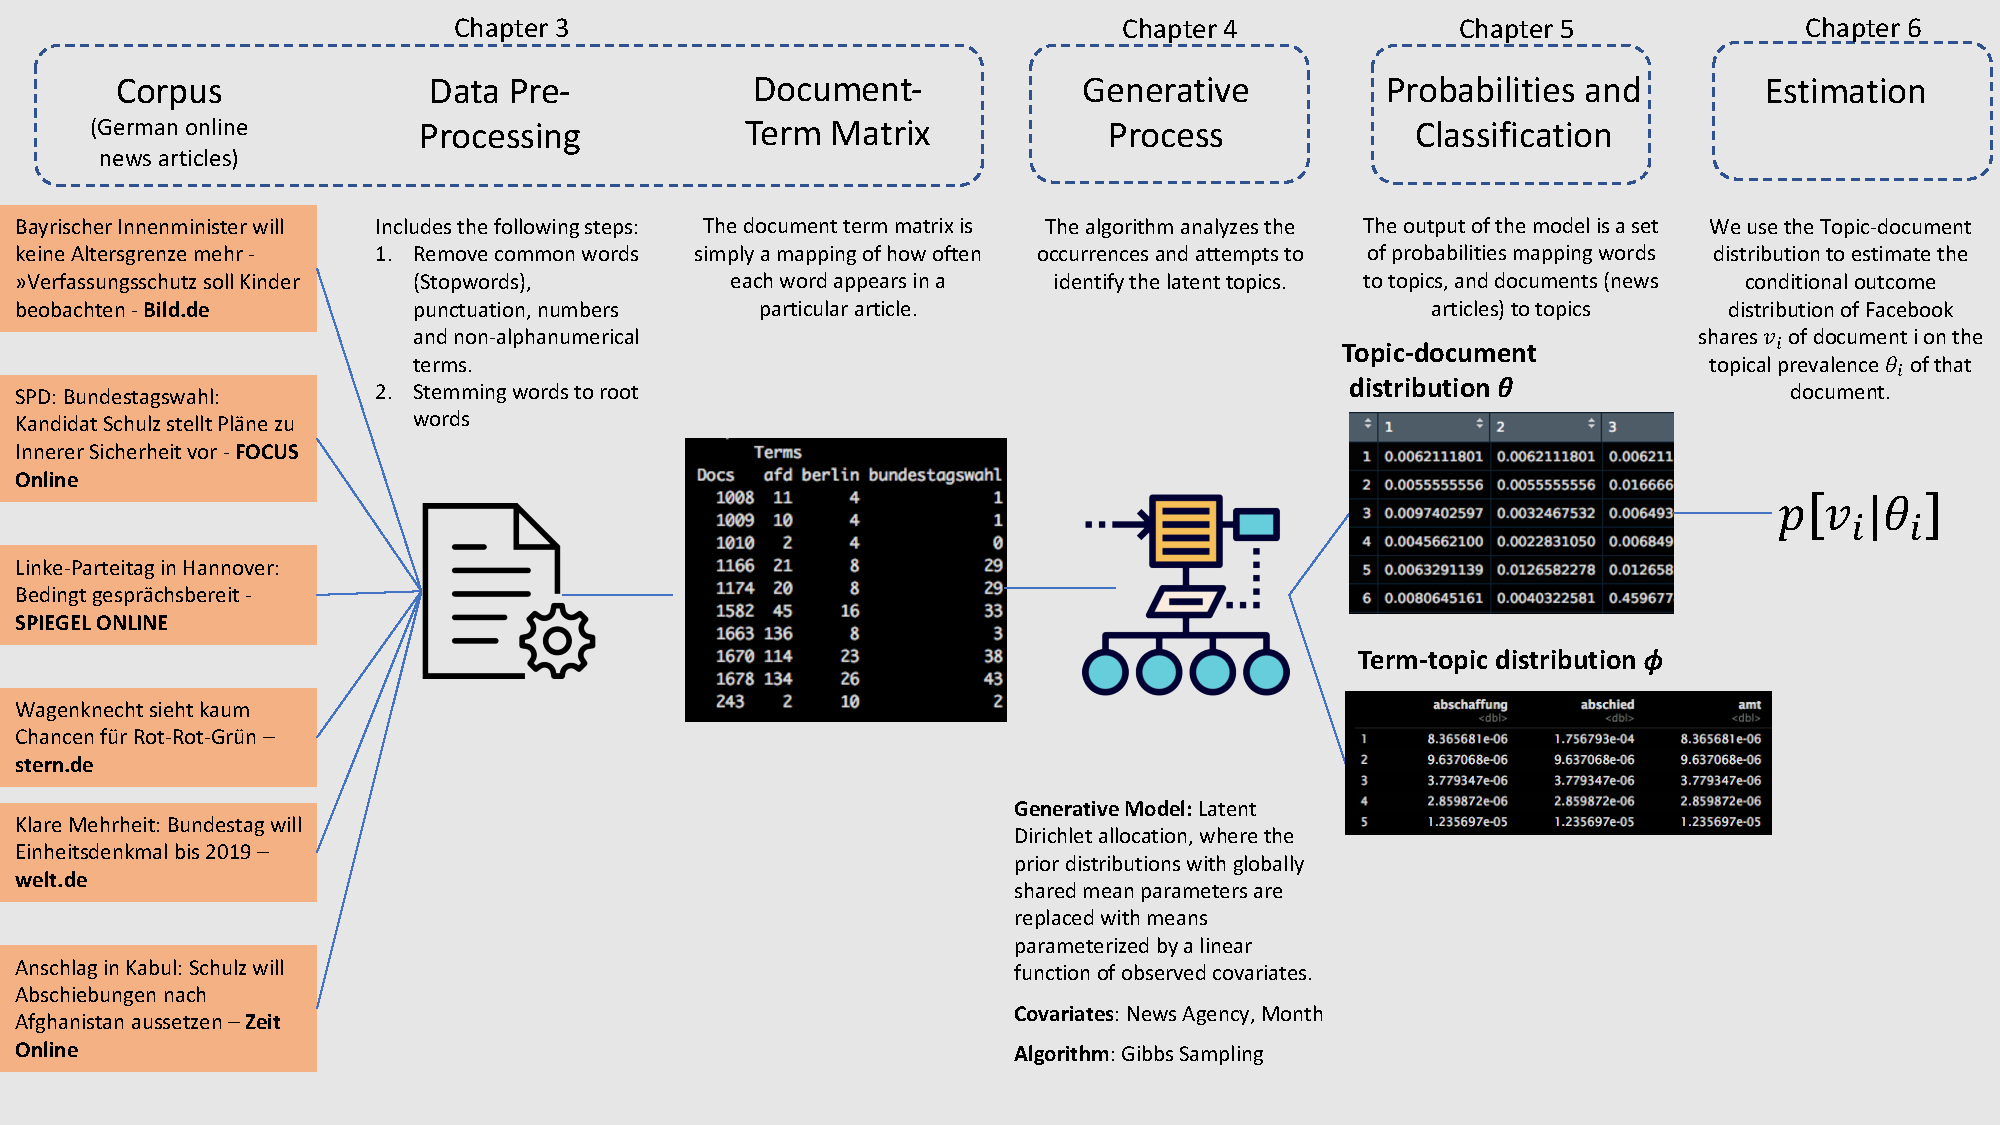
\includegraphics[width=0.95\textwidth]{../figs/research_strategy.pdf} 
	\caption{Research Strategy}
	\label{fig_research_strat}
\end{figure}

% Related Literature
% ------------------
\section{Related Literature}
% ---------------------------------------
% Business Model in the online news market
% --------------------------------------- 
\subsection{The online news market}

Media outlets naturally appear as two-sided platforms, that allow interaction between two categories of consumers: audiences and advertisers. As the demand on both consumer-sides are linked via indirect network externalities, the market in which media outlets operate are referred to as two-sided or multi-sided markets. The theoretical literature on two-sided markets originates from the analysis of credit card markets \citep{rochet_platform_2003} and was later transferred to the concept of other industries, such as dating agencies, real estate agents, and internet “business-to-business” websites \citep{caillaud_chicken_2003}. The basic concept of two-sided markets was already discussed decades ago in several economic studies, especially on media markets \citep{corden_maximisation_1952}, \citep{gustafsson_circulation_1978}, \citep{blair_pricing_1993}. However, comprehensive analyses have only been carried out in the last ten years, starting with the works of \citet{rochet_platform_2003}, \citet{evans_empirical_2003} and \citet{armstrong_competition_2006}.

Advertising-supported media such as online newspapers are typical examples of two-sided markets where the newspaper can be conceived as platforms that allow interaction between audiences ("eyeballs") and advertisers. The newspaper creates (or buys) content to attract viewers which in turn attract advertisers who pay for readers' attention.\cite{evans_industrial_2005} The size and characteristics of the audience has a positive effect on the advertisers' willingness to pay, as advertisements are typically sold based on cost per viewer, often expressed in terms of the cost of reaching a thousand viewers (CPM). Advertising can also have an effect on the recipients, which can be both negative and positive, depending on the quality of the advertising. Depending on the strength of the indirect network effects, private publisher maximize their revenue by balancing the demand from advertisers and subscribers using different business models \citep{evans_economics_2008}.\footnote{Public media such as Tagesschau.de do not depend on revenues from the advertising industry, which means that there is no two-way market structure.} Many traditional newspapers follow the subscription/advertising model, where the publisher charges both market sides: The audience pays a fee to obtain access to the content, and advertisers pay to obtain access to the viewers. Many online news agencies provide part of their editorial content for free and hide another, more exclusive part behind a paywall. However, since the Internet has considerably simplified the possibilities for obtaining information and thus reduced the marginal utility of content, such a business model can only be efficient if the content is very exclusive. As a result, many publishers rely on a free-media model, in which the publishers do not charge viewers for access to the media at all, in order to attract as many eyeballs as possible to their platform, and thus exploit the indirect network effects on the advertising site. In fact, most advertising-financed online magazines earn their gross margin from advertising.\cite{evans_industrial_2005} In order to maximize their profits, these companies have an interest in attracting as many readers as possible. Facebook is an important traffic supplier for news sites: Over 487.000 news articles from TOP15\footnote{Bild.de, bunte, Chip, FAZ, Focus, Handelsblatt, Heise, N-TV, Spiegel, Sport1, Stern, Süddeutsche, Tagesschau, Welt, Zeit} media were shared 123.000.000 times on Facebook (94\%), Twitter(3.5\%) and Google+(2.3\%).\cite{schiller_development_2016} In addition to the quantity of the audience, the demographic characteristics of recipients also have an influence on the willingness to pay on the advertiser site. Online advertising makes it possible to target ads to particular consumers in real time. Facebook instant articles facilitates this targeting, as they make the public users profile data available to the publisher. However, not all topics are equally often distributed in social media. \citet{schiller_development_2016} show, that social media users choose a certain site depending on the researched topic. FOCUS Online for example is targeted for articles from politics and business, while sports news is more likely to be shared from Bild.de. 

While these pre-defined resorts give an indication on the content of an article, multiple articles in the same resort probably don't cover the same topics. Especially if the articles originate from different news portals. Furthermore, articles can contain more than one topic. We use a structural topic model to reveal the underlying topics of a collection of articles, and how the articles exhibit them. We then estimate the effect of topic prevalence on the number of Facebook shares. We use a data set of online news articles about domestic politics dated from 01.06.2017 to 22.11.2017\footnote{German federal elections took place on 24th of September 2017.} from seven German content providers: Bild.de, Die Welt, Focus Online, Spiegel Online, Stern.de, Zeit Online and Tagesschau.de. They are all providers of online news, whereby Tagesschau.de is the only publicly funded service. The latter was also included in the study to verify whether the topics differ when the content is created on the basis of a different business model. 

Figure \ref{fig_uuser} shows the coverage of the six private online news provider for the period June to November 2017 in terms of unique user.\footnote{The Term unique user refers to the number of different internet users who have visited the website within a certain period of time. The unique user is the basis for the calculation of coverage and structures of online advertising media as well as essential factors for media planning.} It is striking that Bild.de has the greatest reach over the entire course of time, except on election day and one day after. Here, DIE WELT (+123\%), FOCUS ONLINE (+71\%) and SPIEGEL ONLINE (+57\%) in particular are making a big leap. SPIEGEL ONLINE overtakes Bild.de (+21\%) on the day after the elections (25.09.2017). ZEIT ONLINE and stern.de have a comparatively small coverage. Yet here too, there is a short-term increase in the range of coverage during the elections (+44\% for stern.de and +81\%  for ZEIT ONLINE).

 % What is the share of advertising revenue in total earnings of german online newspaper ? 

\begin{figure}[H]
	\caption{Unique User in Million}
	\begin{center}
			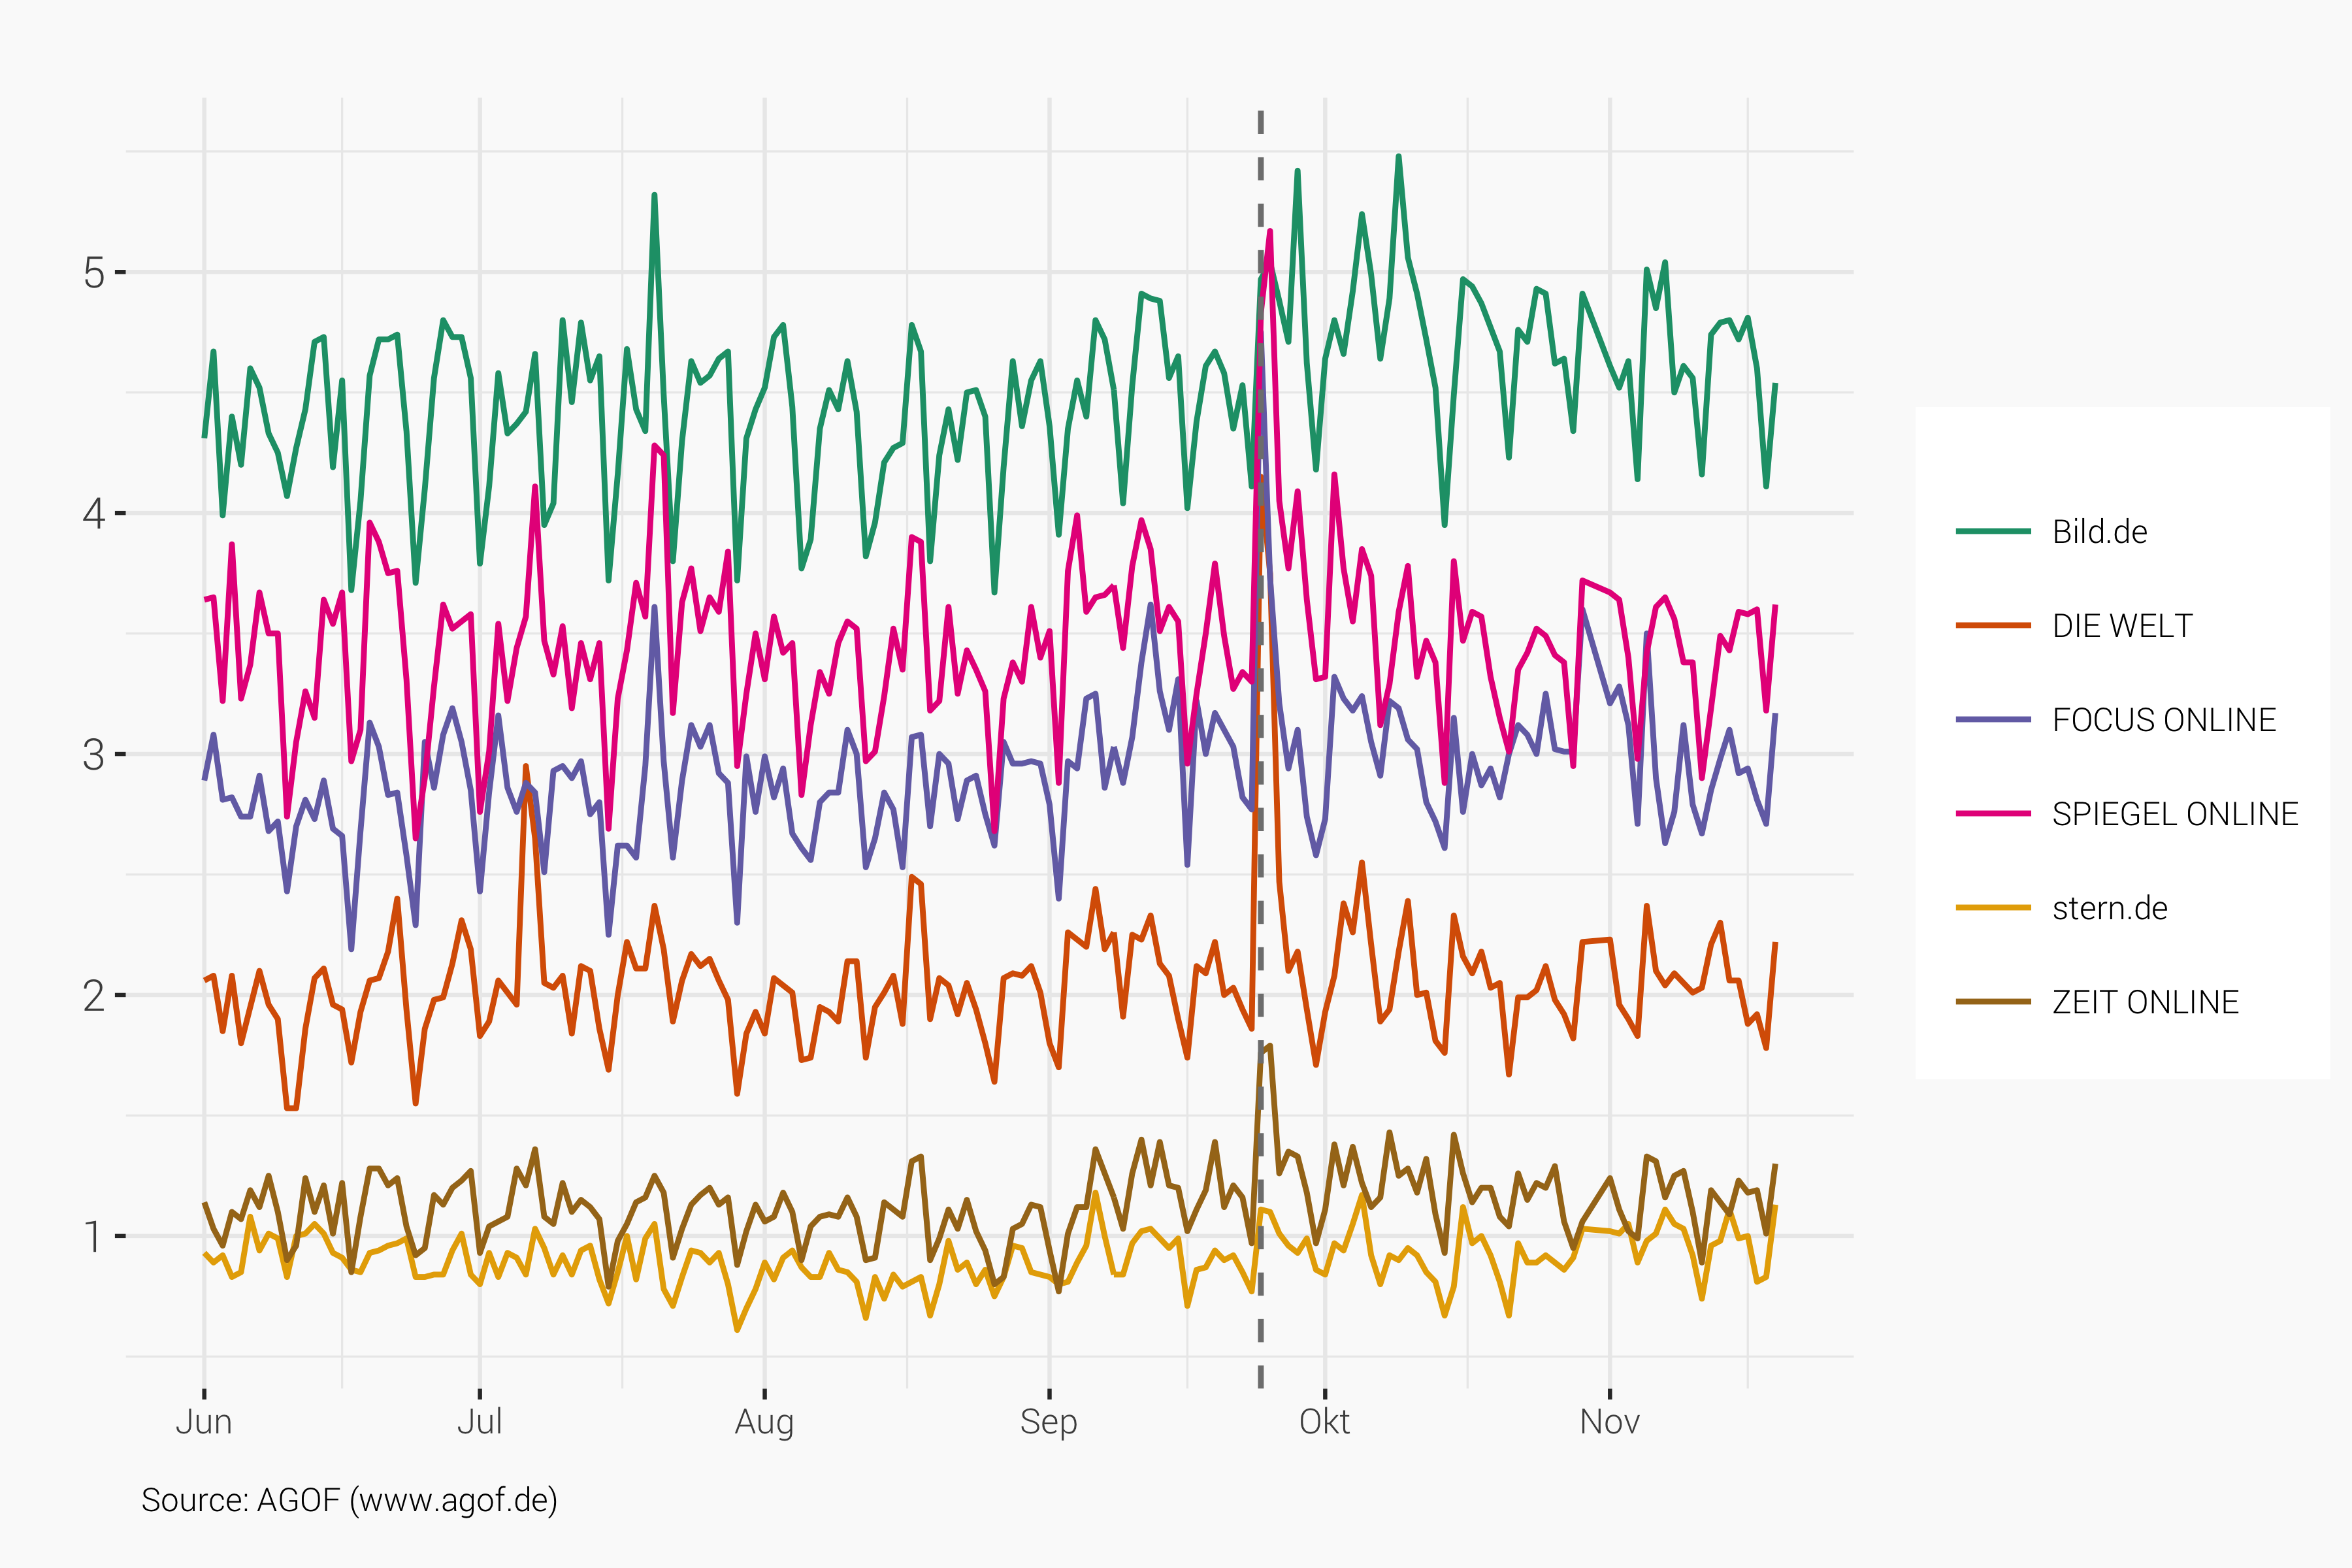
\includegraphics[width=.9\textwidth]{../figs/uniqueUser.png}
			\label{fig_uuser}
	\end{center}
\end{figure}

 

The two-sided market structure of news markets results in news platforms striving to choose their content in such a way that its reach is as large as possible in order to maximize profits from advertising revenues. This may lead to media-bias, as advertising may affect the ability and incentives of media to provide independent news. On the other hand, advertising may also have a positive impact on the media, as it enables publishers to report independently of political parties. \citet{ellman_what_2009} found that advertising increases the intensity of competition for readers and therefore raises accuracy of media coverage. 

% --------------
% Topic Modeling
% --------------
\subsection{Topic Modeling}

We use the structural topic model (STM) developed by \citet{roberts_model_2016} that allows us to incorporate document specific covariates (e.g. the author or date of a document). STM is a recent extension of the standard topic modeling technique, labeled as "latent Dirichlet allocation" (LDA), which refers to the Bayesian model in \citet{blei_latent_2003} that treats each word in a topic and each topic in a document as generated from a Dirichlet - distributed prior.\footnote{See also \citet{griffiths_probabilistic_2002}, \citet{griffiths_finding_2004} and \citet{hofmann_probabilistic_1999}. \citet{pritchard_inference_2000} introduced the same model in genetics for factorizing gene expression as a function of latent populations.} Topic models formalize the idea that documents are formed by hidden variables (topics) that generate correlations among observed terms. Since its introduction into text analysis, LDA has become hugely popular and especially useful in political science.\footnote{see \citet{blei_probabilistic_2012}, \citet{grimmer_text_2013} and \citet{wiedmann_text_2016} for an overview in social science and \citet{gentzkow_text_2017} give an overview of text mining applications in economics.} \citet{wiedmann_text_2016} use topic model methods in on large amounts of news articles from two german newspapers published between 1959 and 2011, to reveal how democratic demarcation was performed in Germany over the past six decades. 

STM has been applied to multiple academic fields: \citet{roberts_structural_2014} uses STM to analyse open-ended responses from surveys and experiments, \citet{farrell_corporate_2016} applies the model to scientific texts on climate change, revealing links between corporate funding and the framing of scientific studies and \citet{mishler_using_2015} shows that "STM can be used to detect significant events such as the downing of Malaysia Air Flight 17" when applied to twitter data. Another study shows how STM can be used to explore the main international development topics of countries’ annual statements in the UN General Debate and examine the country-specific drivers of international development rhetoric \citep{baturo_what_2017}. \citet{mueller_reading_2016} uses newspaper text to predict armed conflicts in different regions. They use the estimated topic shares in linear fixed effects regression to forecast conflict out-of-sample.

% -----
% Data
% -----
\section{Dataset}\label{ch_data}

We conduct our estimation on a sample of 10531 online news articles from seven news provider about domestic politics dated from 01.06.2017 to 22.11.2017.\footnote{German federal elections took place on 24th of September 2017.} We first extract all online articles of six mainstream german online news portals\footnote{Bild.de, Focus.de, Spiegel.de, Stern.de, Welt.de, Zeit.de, Tagesschau.de} using the the Event Regestry API.\footnote{For more information see http://eventregistry.org/documentation. The scraping code was written in Python and can be made available on request.} We then filtered all articles from the section "domestic policy" by checking the URL structure. We used the URL of these articles, to check how many times they where shared on Facebook using the \textit{sharedcount} API.\footnote{http://docs.sharedcount.com/} The returned share count is the sum of (1) the number of likes of this URL, (2) the number of shares of this URL (including copy-pasting a link back to Facebook), (3) the number of likes and comments on stories on Facebook about this URL and (4) the number of inbox messages containing this URL as an attachment.\footnote{See https://developers.facebook.com/docs/graph-api for more information about the Facebook Graph API.}

Figure \ref{fig_distr1}\footnote{The first vertical line indicate the date of the federal elections (24.09.2017), and the second line indicate the date on which the "Jamaika" parties (Union, FDP, Die Grünen) announced the failure of the coalition negotiations (20.11.2017).} shows the distribution of the number of articles from the respective news sources by date. There is a high peak around the federal elections on September, 24th. Most of the articles are published by welt.de, followed by stern.de (see \ref{fig_distr2}).  

\begin{figure}[H]
	\caption{Article distribution...}
	\begin{center}
		\begin{subfigure}[normla]{0.8\textwidth}
			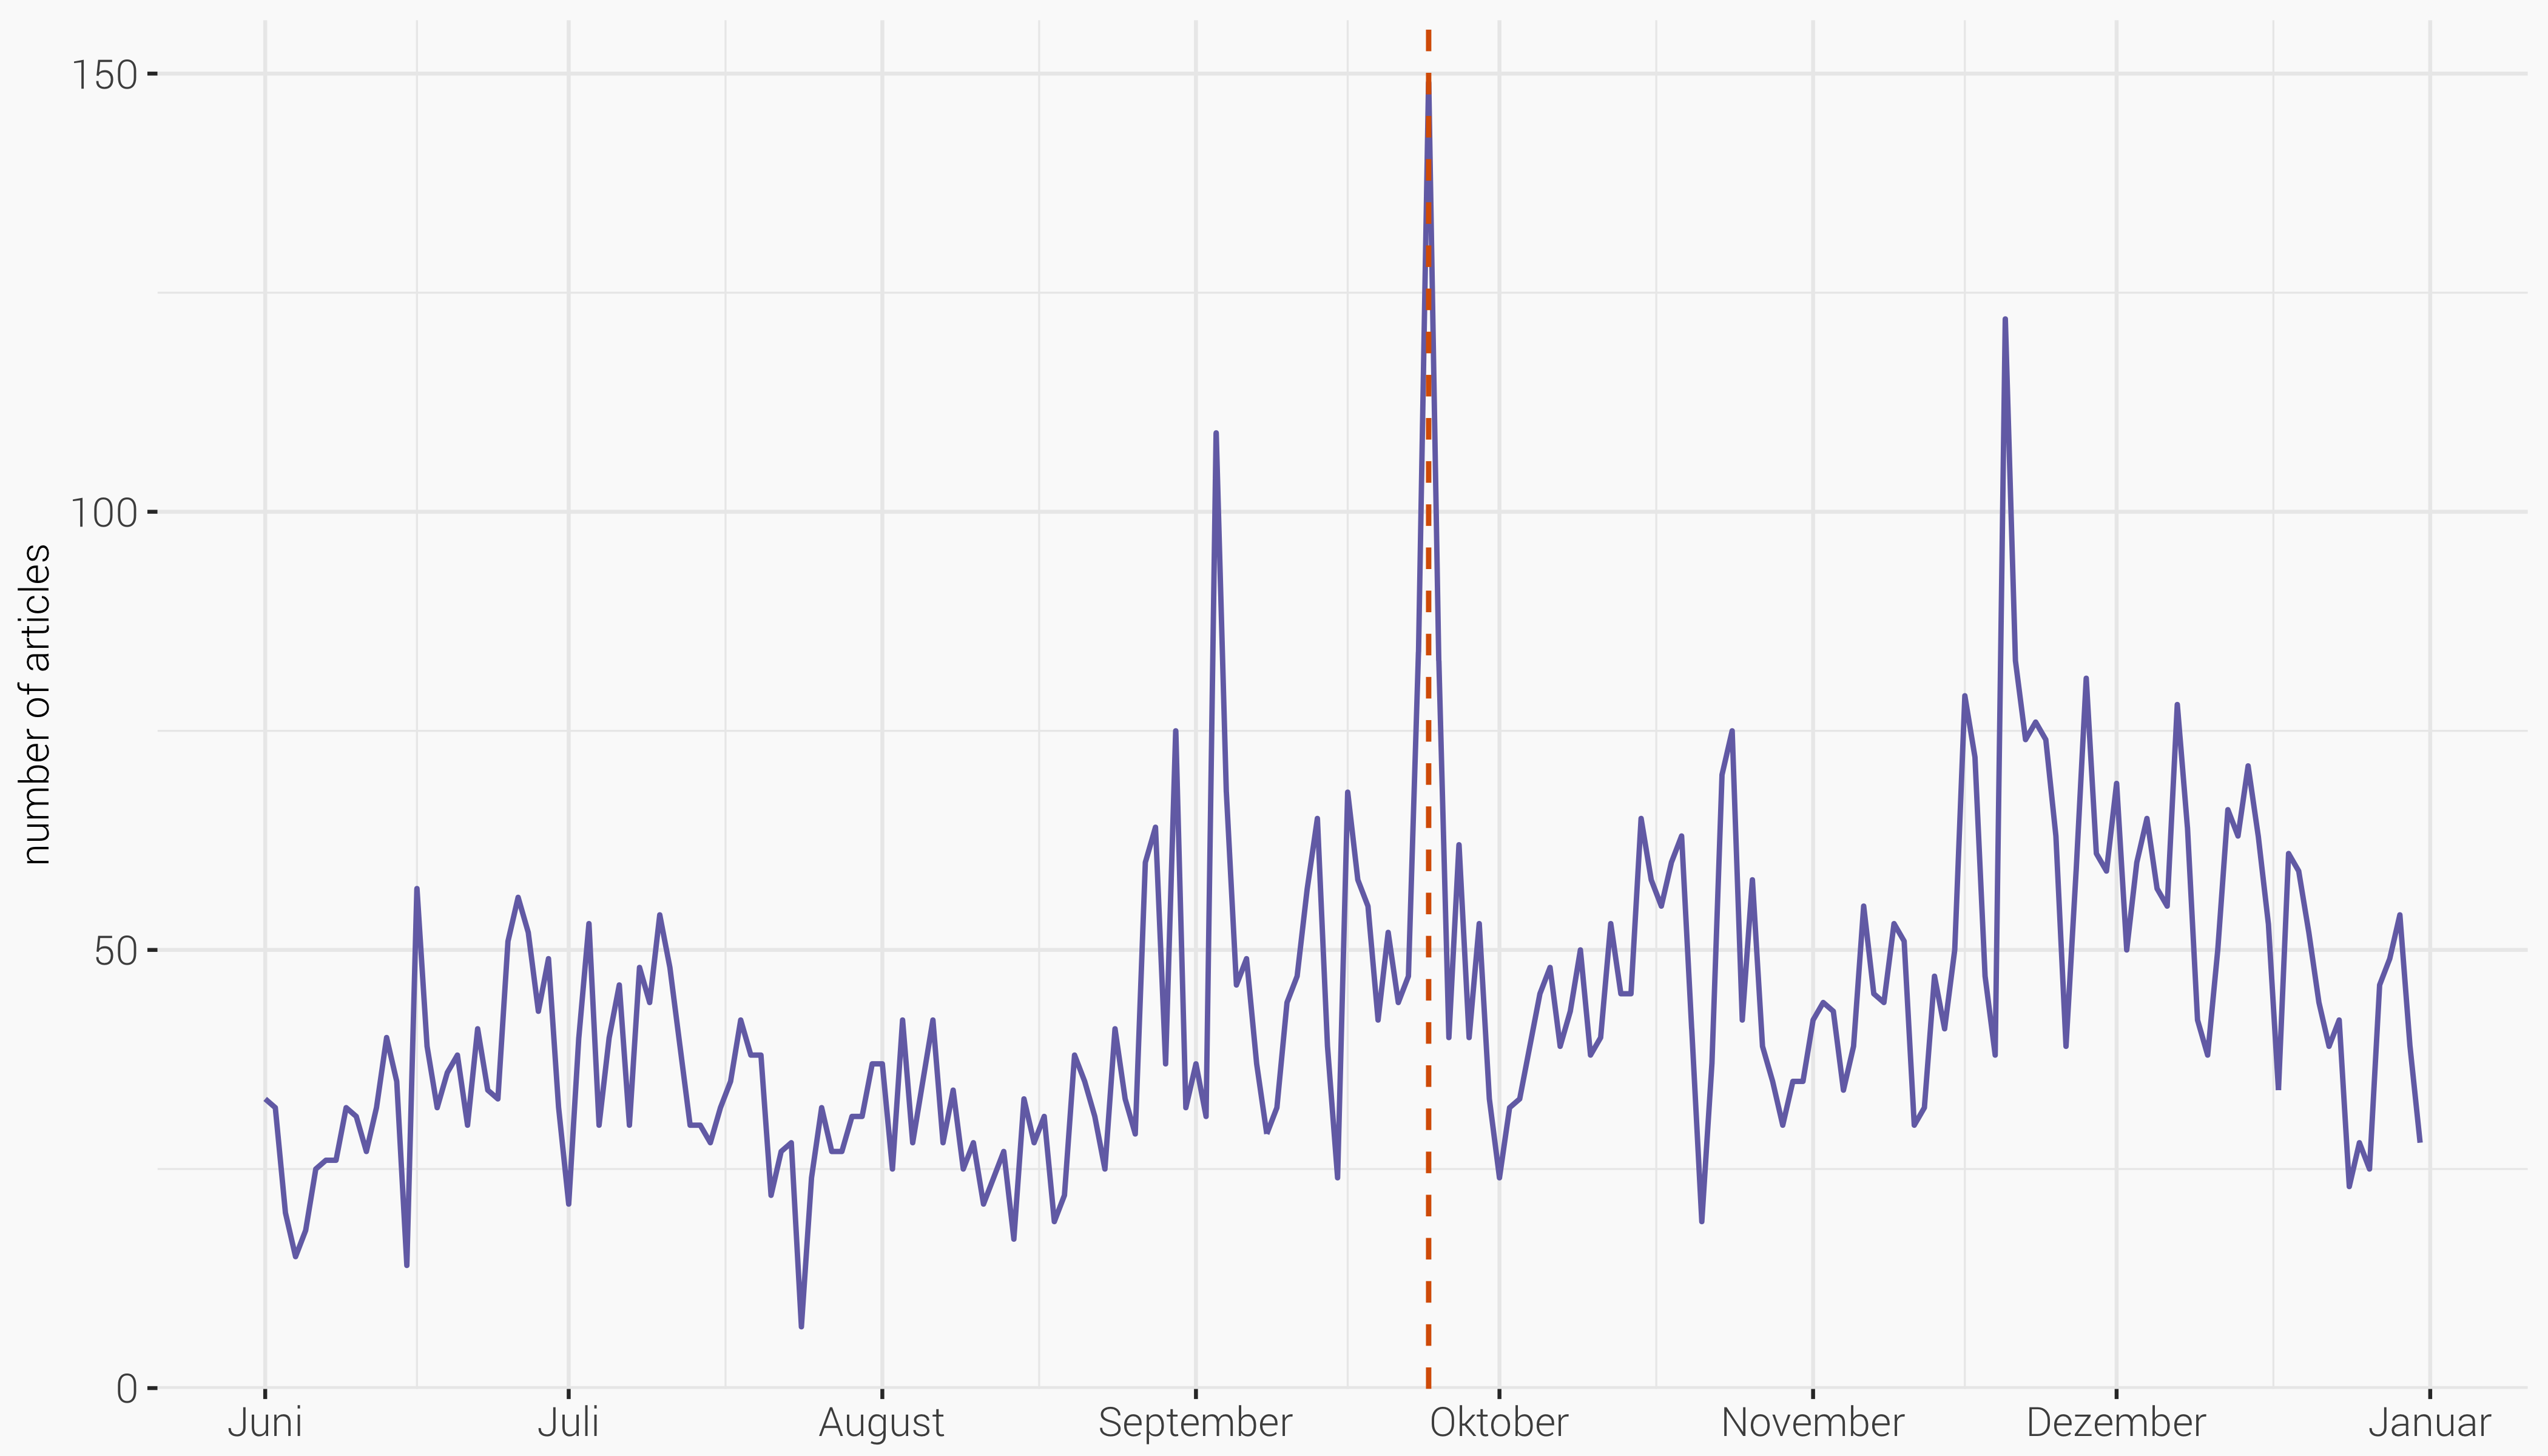
\includegraphics[width=\textwidth]{../figs/timeline.png}
			\caption{...by date \& news source}
			\label{fig_distr1}
		\end{subfigure}
		\begin{subfigure}[normla]{0.8\textwidth}
			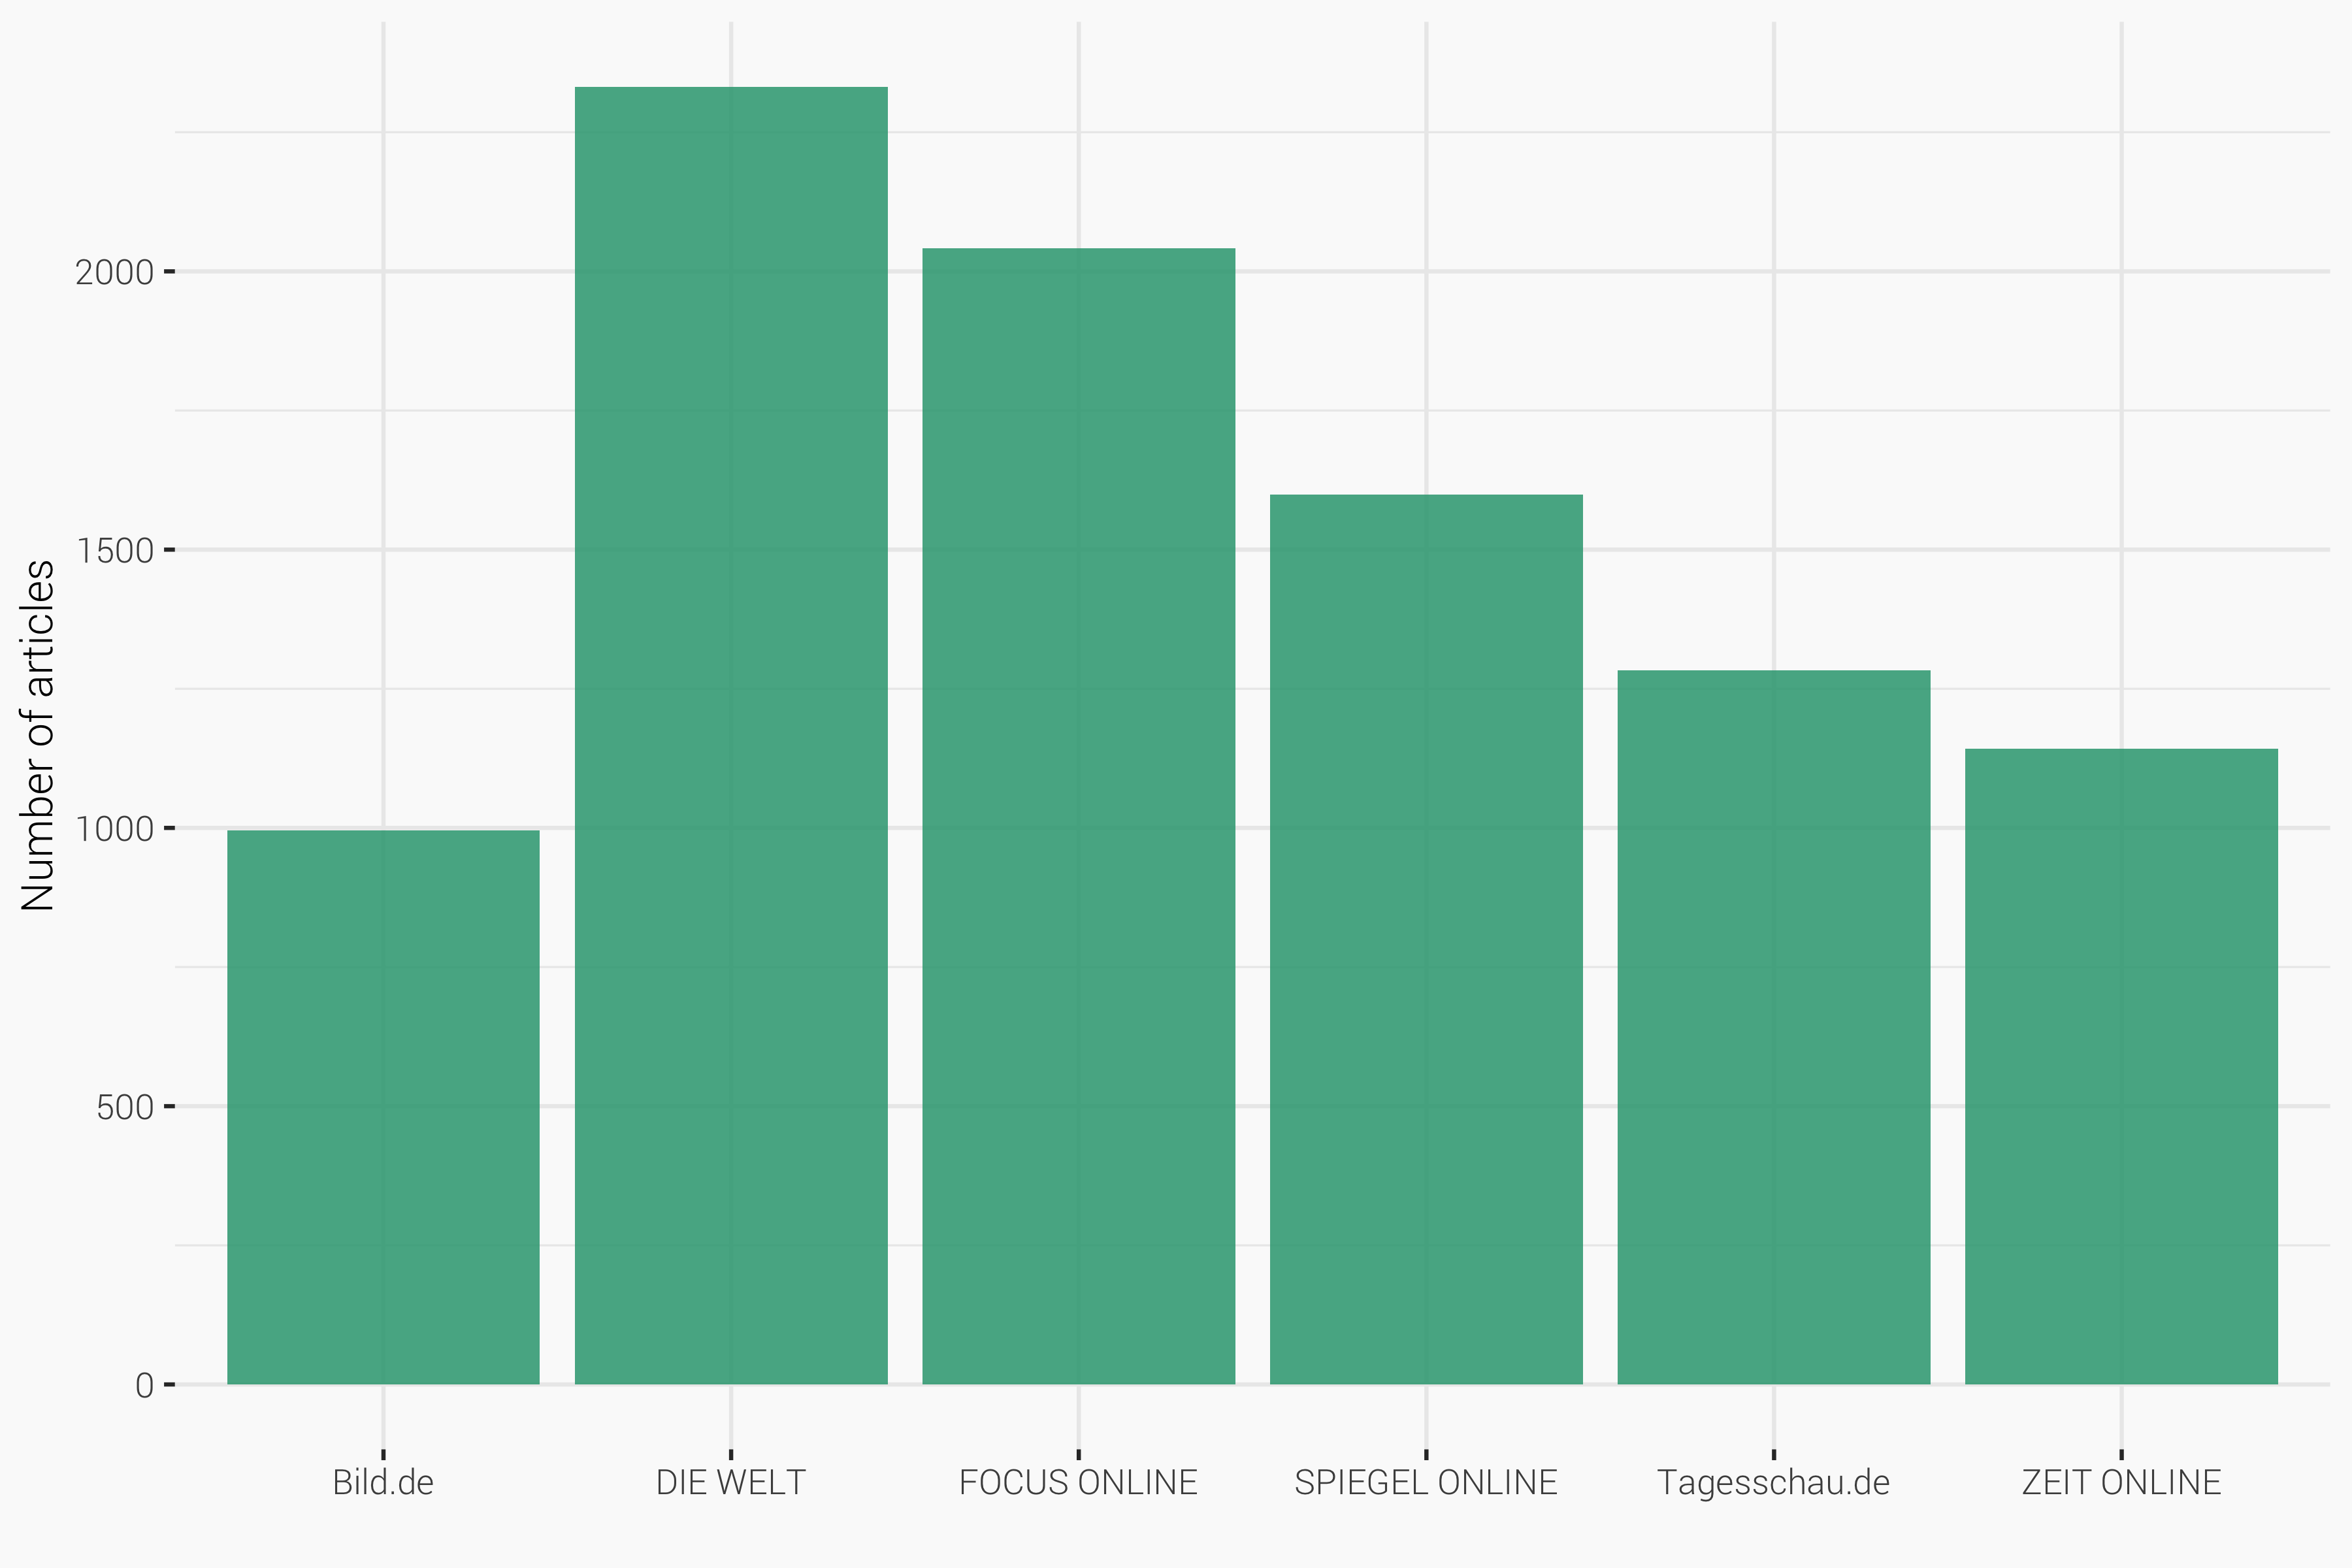
\includegraphics[width=\textwidth]{../figs/bar.png}
			\caption{... by news source}
			\label{fig_distr2}
		\end{subfigure}
	\end{center}
\end{figure}

% ------------------
% Text Pre-Procesing
% ------------------

To use text as data and reduce the dimensionality, a common strategy is to pre-process the text by imposing some preliminary restrictions (stop-word removal, tokenization) based on the nature of the data (twitter text, newspaper articles, speeches, etc.) to reduce the number of language elements to consider \citep{gentzkow_text_2017}. An overview of how these steps were applied to our data set can be found in the next section. 

After pre-processing, each document $d$ is a finite list of terms. Each unique term in the corpus is indexed by some $v \in \lbrace 1,...,V \rbrace$ where $V$ is the number of unique terms. For each document $d \in \lbrace 1,...,D \rbrace$ we compute the number of occurrences of term $v$ in document $d$ to obtain the count $x_{d,v}$. The $D$ x $V$ matrix $\boldsymbol{X}$ of all such counts is called the document-term matrix. This representation is often referred to as the bag of words model, since the order in which words are used within a document is completely disregarded. 

A central task in text mining is to extract low-dimensional information from documents that are high-dimensional by nature \citep{bholat_text_2015}. This is related to the task of reducing the number of unique language elements in order to reduce the dimensionality of data (to avoid unnecessary computational complexity and overfitting) while at the same time keeping those words that reflect the content of a document. Any useful representation of text will throw away some information, the trick is to include the relevant information for our needs, and exclude the extraneous information. 

Intuitively the term frequency (tf) of a word is a measure of how important that word may be. There are words in a document, however, that occur many times but may not be important like articles, conjunctions, and so on. These terms, often called "stop words", are important to the grammatical structure of a text, but typically don't add any additional meaning and can therefore be neglected. We use a pre-defined stop word list from the Snowball stemmer project\footnote{http://svn.tartarus.org/snowball/trunk/website/algorithms/*/stop.txt} together with a customized list of stop-words that are redundant superfluous or distorting. We also remove punctuation character (e.g. ., ,, !, ?, etc.) and all numbers from our corpus.  

% ----------------------
% Structural topic Model
% ----------------------
\section{Topic detection using the structural topic model}\label{ch_model}

The following description of the generative model of the STM is based on \citet{roberts_structural_2013} and \citet{roberts_stm:_2016}. The process of filling a word-position in a document begins with the generation of a document-specific topic-prevalence vector $d(\boldsymbol{\theta}_d)$ drawn from a logistic-normal distribution, where the parameters are a function of the covariate values:

\begin{align*}
	\boldsymbol{\theta}_d|\boldsymbol{x}_{d\gamma},\boldsymbol{\Sigma} \sim \textrm{LogisticNormal}(\mu = \boldsymbol{x}_{d\gamma}\boldsymbol{\Sigma})
\end{align*}

$\boldsymbol{x}_d\gamma$ lists the values of all metadata covariates for document $d$, where $\gamma$ relates these covariate values to the topic-prevalence. The structure of $\boldsymbol{\Sigma}$ implies the possibility of correlations across documents in the topic-prevalence vector which help enhance interpretation and prevent overfitting. 

Given the document-specific distribution over topics, for each word in the document ($n \in \lbrace 1,...,N_d\rbrace$) is assigned to a specific topic $z_{dn}$ through the process

\begin{align*}
	z_{dn}|\boldsymbol{\theta}_d \sim \textrm{Multinomial}(\boldsymbol{\theta}_d)
\end{align*}

where the $k^{th}$ element if $z_{dn}$ is unity and all other elements are zero when topic $k$ is chosen. 

Conditional in the topic chosen, a specific word, $w_{dn}$, is chosen from the overall corpus vocabulary $V$ to fill position $n$ in document $d$, using the following process:

\begin{align*}
	w_{dn}|z_{dn},\beta_{dkv} \sim \textrm{Multinomial}(\beta_{dk1},...,\beta_{dkV}).
\end{align*}

where the word probability $\beta_{dkv}$ is modeled as a function of the two parameters $m_v$ (indicating the importance of that word across all documents) and $\kappa_{kv}$ (indicating the importance of the word given the topic $k$). Transforming the sum of these coefficients into probabilities for use in a multinomial distribution via logistic transformation, one obtains:

\begin{align*}
	\beta_{dkv}|z_{dn}\propto\textrm{exp}(\boldsymbol{m}_v+\kappa_{kv})
\end{align*}


% ----------------------
% Model Selection
% ----------------------
\subsection{Model and parameter selection}

Topic models are usually imprecise as a number of assumptions have to be made that influence the performance of the classification task. Furthermore, multiple solutions exist for the optimization problem. The STM maximizes the posterior likelihood that the observed data were generated by the above data-generating process using an iterative approximation-based variational expectation-maximization algorithm\footnote{A technical description of this maximization process can be found in \citet{roberts_model_2016}} available in R's stm package \citep{roberts_stm:_2016}. Regularizing prior distributions are used for $\gamma$, $\kappa$ and $\Sigma$. Since an ex ante valuation of a model is hardly possible, we compute a variety of different models with different parameters and compare them with respect to the research problem \citep{gentzkow_text_2017}. To evaluate the accuracy of a model its perplexity can be computed. Similar to cross-validation (VC), different model specifications are compared to how well they do in predicting words within a document \citep{asuncion_smoothing_2012}, \citep{wallach_evaluation_2009}. However, \citet{chang_reading_2009} have proven with large user studies that optimal held out likelihood does not correspond to human perception of semantic coherence of topics. \cite{mimno_optimizing_2011} introduced a measure of coherence of a topic by observing co-occurences of the top $N$ terms of each topic on a document. Another strategy for selecting an appropriate model is to check for residual overdispersion of the variance of the multinomial within the data generating process of the model \citep{taddy_estimation_2012}. Other approaches can be found in \citet{airoldi_reconceptualizing_2010} and \citet{teh_hierarchical_2006}. However, cross-checking some subset of assigned topic distributions to evaluate whether the estimates align with the concept of interest \citep{gentzkow_text_2017}. We apply these manual audits together with numeric optimization based on the topic coherence measure suggested by \citet{mimno_optimizing_2011}. 

This process revealed that a model with 25 topics best reflects the structure in the corpus. Furthermore, we use the source of each article (the media house) and the month it was published as covariates in the topic prevalence portion of the model. In other words, the probability distribution of topics depends on the editorial strategy of a media house as well as on the month the article was published. To address problems due to non-convexity, we rely on the spectral initialization approach advocated by \citet{roberts_navigating_2016}. 

% ----------------------
% Model Results
% ----------------------
\subsection{Visualize model results}

To get a first overview of the semantic concept of the topics, we produce a random sample of posts with a comparatively high posterior probability for that topic (see \ref{fig_classification}). Figure \ref{fig_topic_proportion} displays the topics ordered by their expected frequency across the corpus. To assign a label to each topic, we used a combination of most frequent words in that topic and words with the highest "score", computed as the log frequency of the word in the topic divided by the log frequency of the word in other topics \citep{roberts_stm:_2016}. The most common topic (3) is a general topic full of words that are frequently used in policy news, and therefore is not very interpretable. However, the remaining labels seem to classify a certain topic.  

\begin{figure}[H]
	\begin{center}
	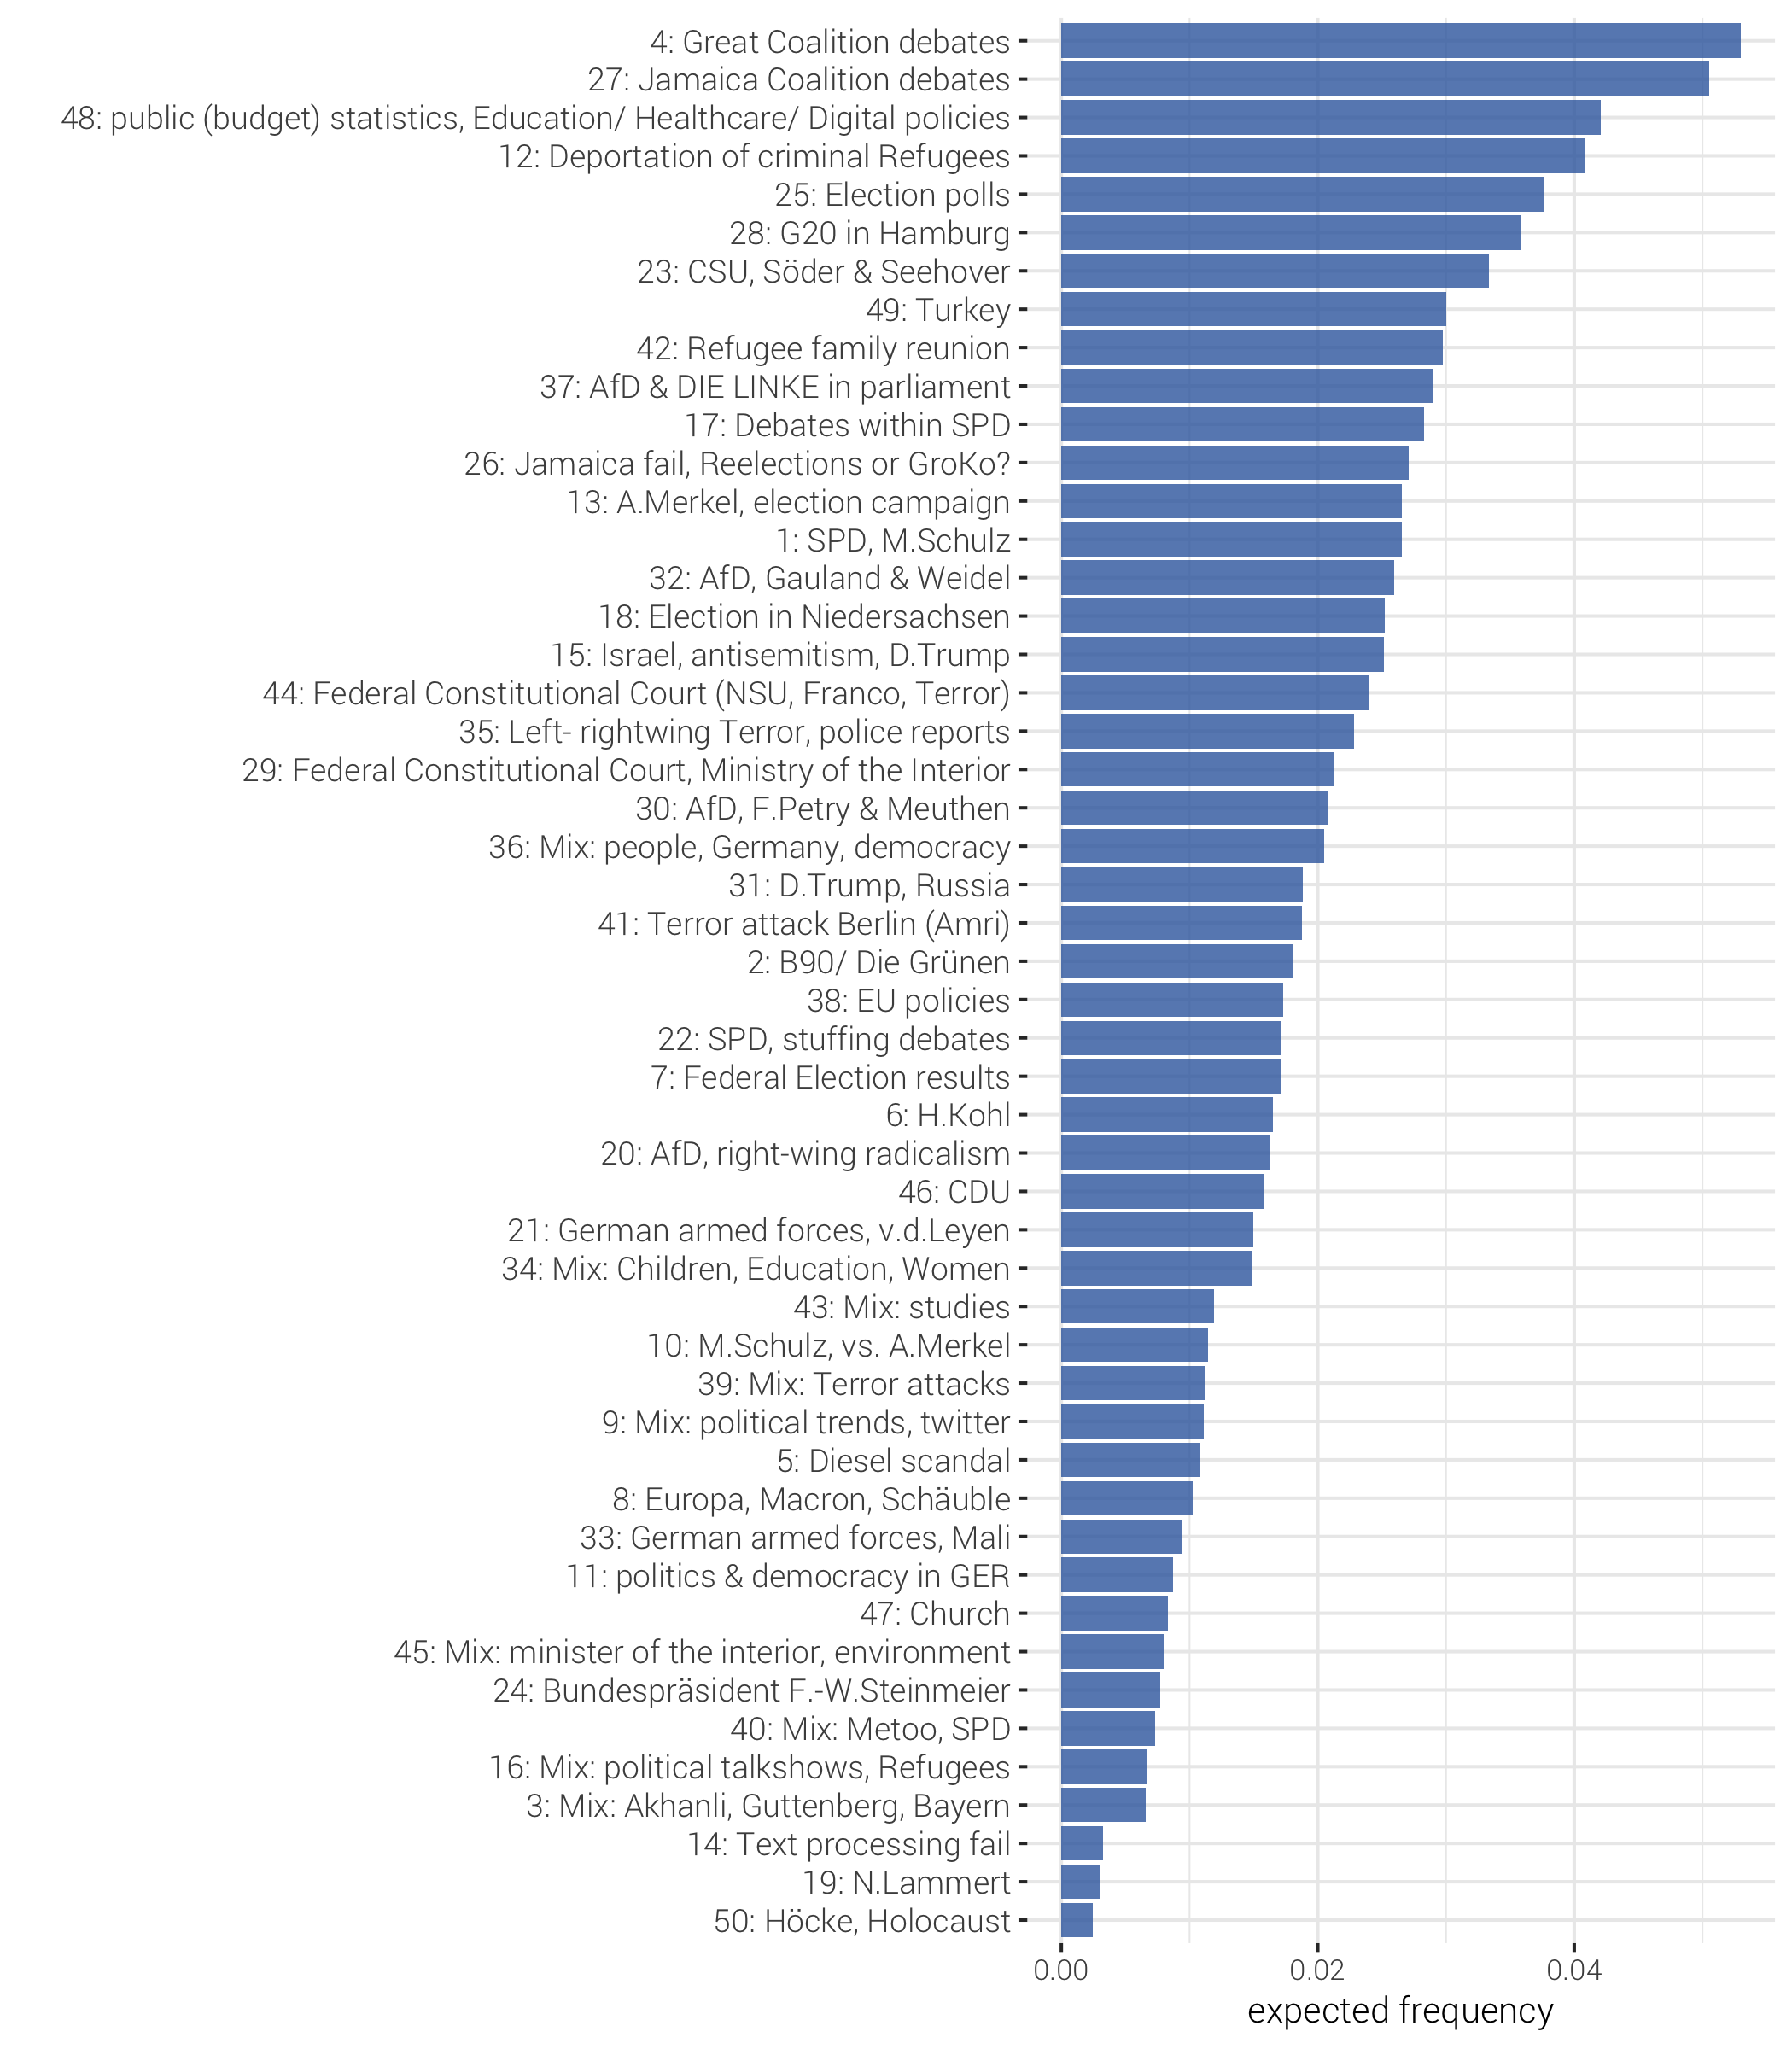
\includegraphics[width=0.8\textwidth,keepaspectratio]{../figs/topic_proportion.png}
	\caption{Expected Topic Proportion}
	\label{fig_topic_proportion}
	\end{center}
\end{figure}

%\begin{landscape}
%\begin{figure}[H]
%\centering
%	\caption{Sample articles}
%	\includegraphics[width=\linewidth,height=.9\textheight,keepaspectratio]{../figs/topic-classification-sample.png}	
%	\label{fig_classification}
%\end{figure}
%\end{landscape}

% ----------------------
% Effect of covariates
% ----------------------
Since we included news source as a covariate in estimating topical prevalence part within the model, we can estimate the frequency a topic is discussed within a news corpus \citep{roberts_model_2016}. We estimate the conditional expectation of topic prevalence for given document characteristics. More specifically, we estimate a linear model, where the documents are observations, the dependent variable is the posterior probability of a topic and the covariates are the metadata of documents. The stm-package provides a function that uses the method of composition to incorporates uncertainty in the dependent variable, drawing a set of topic proportions from the variational posterior repeated times and compute the coefficients as the average over all results. 

Figure \ref{fig_estimateEffects_small} displays topics, where the most significant differences between the news sources are discernible.\footnote{An overview of all estimated topics can be found in the appendix \ref{fig_estimateEffects_full1} and \ref{fig_estimateEffects_full2}.} Topic 2, classifying articles about the diesel scandal, the glpyphosate decision and green policies, occur comparatively more often in tagesschau.de and bild.de, whereas tagesschau.de reports comparatively little about the riots during the G20 summit (topic 9). Topics 10 (about public (financial) statistics) and 13 (about the federal migration office (BAMF), asylum procedures and other issues related to refugees) also seems to be represented comparatively frequently in the tagesschau.de corpus, the latter topic is most often discussed in the DIE WELT corpus. However, topic 20 (the public debate between Die Grünen and FDP in the process of coalition negotiations) is represented significantly more often in the corpus of spiegel.de and bild.de. Topic 26, which classifies articles that deal with terrorism, mainly about the NSU trial and the main defendant Zschäpe as well es IS, is significantly more often present in the corpus of FOCUS ONLINE.

\begin{figure}[H]
	\caption{Mean prevalence of topics within each news source corpus}
	\begin{center}
		\begin{subfigure}[normla]{0.3\textwidth}
			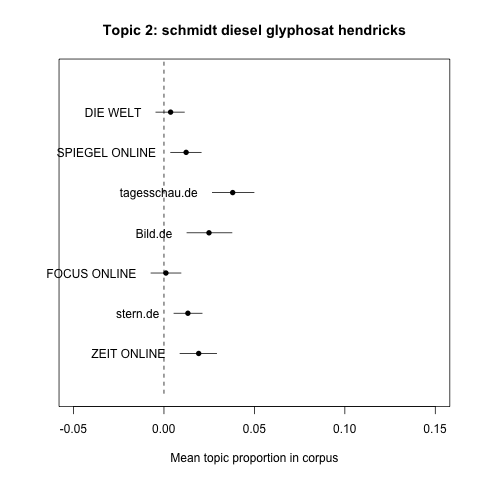
\includegraphics[width=\textwidth]{../figs/estimate_effect2.png}
		\end{subfigure}
		\begin{subfigure}[normla]{0.3\textwidth}
			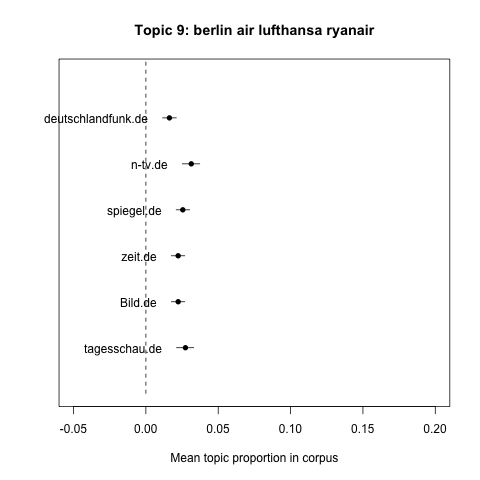
\includegraphics[width=\textwidth]{../figs/estimate_effect9.png}
		\end{subfigure}
				\begin{subfigure}[normla]{0.3\textwidth}
			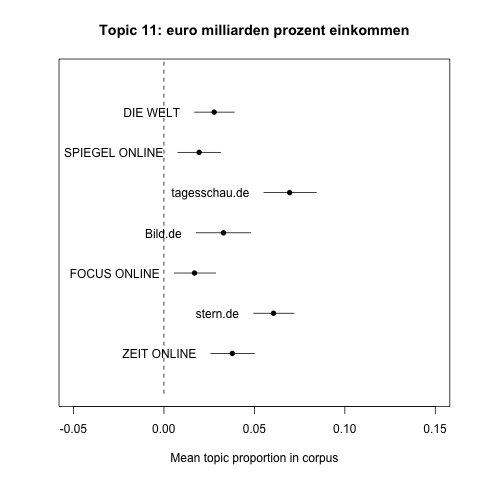
\includegraphics[width=\textwidth]{../figs/estimate_effect11.png}
		\end{subfigure}
				\begin{subfigure}[normla]{0.3\textwidth}
			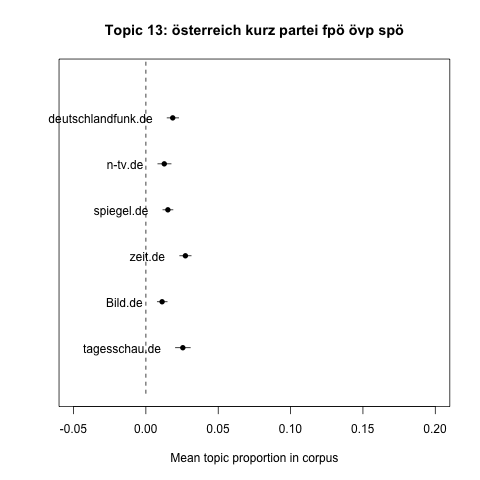
\includegraphics[width=\textwidth]{../figs/estimate_effect13.png}
		\end{subfigure}
				\begin{subfigure}[normla]{0.3\textwidth}
			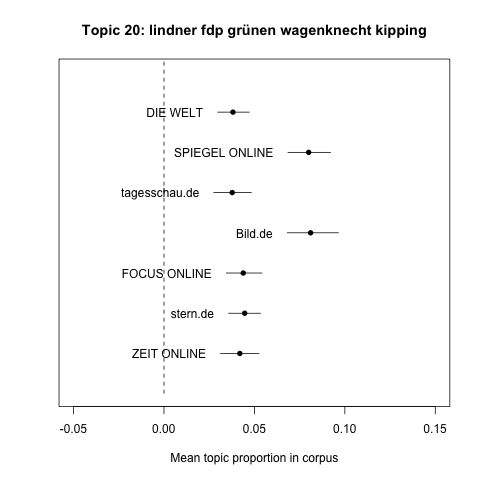
\includegraphics[width=\textwidth]{../figs/estimate_effect20.png}
		\end{subfigure}
				\begin{subfigure}[normla]{0.3\textwidth}
			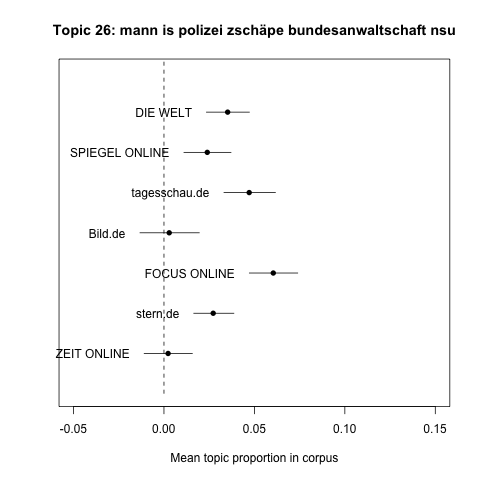
\includegraphics[width=\textwidth]{../figs/estimate_effect26.png}
		\end{subfigure}
	\end{center}
	\label{fig_estimateEffects_small}
\end{figure}

Another interesting aspect is how the news sources discusses the different topics, that is, describe the same event with different vocabulary.


% ----------------------
% Regression
% ----------------------
\section{Causal relationship between topics and social media shares.}\label{ch_regression}

%\begin{figure}[H]
%\centering
%	\caption{Sum of Facebook shares by topic}
%	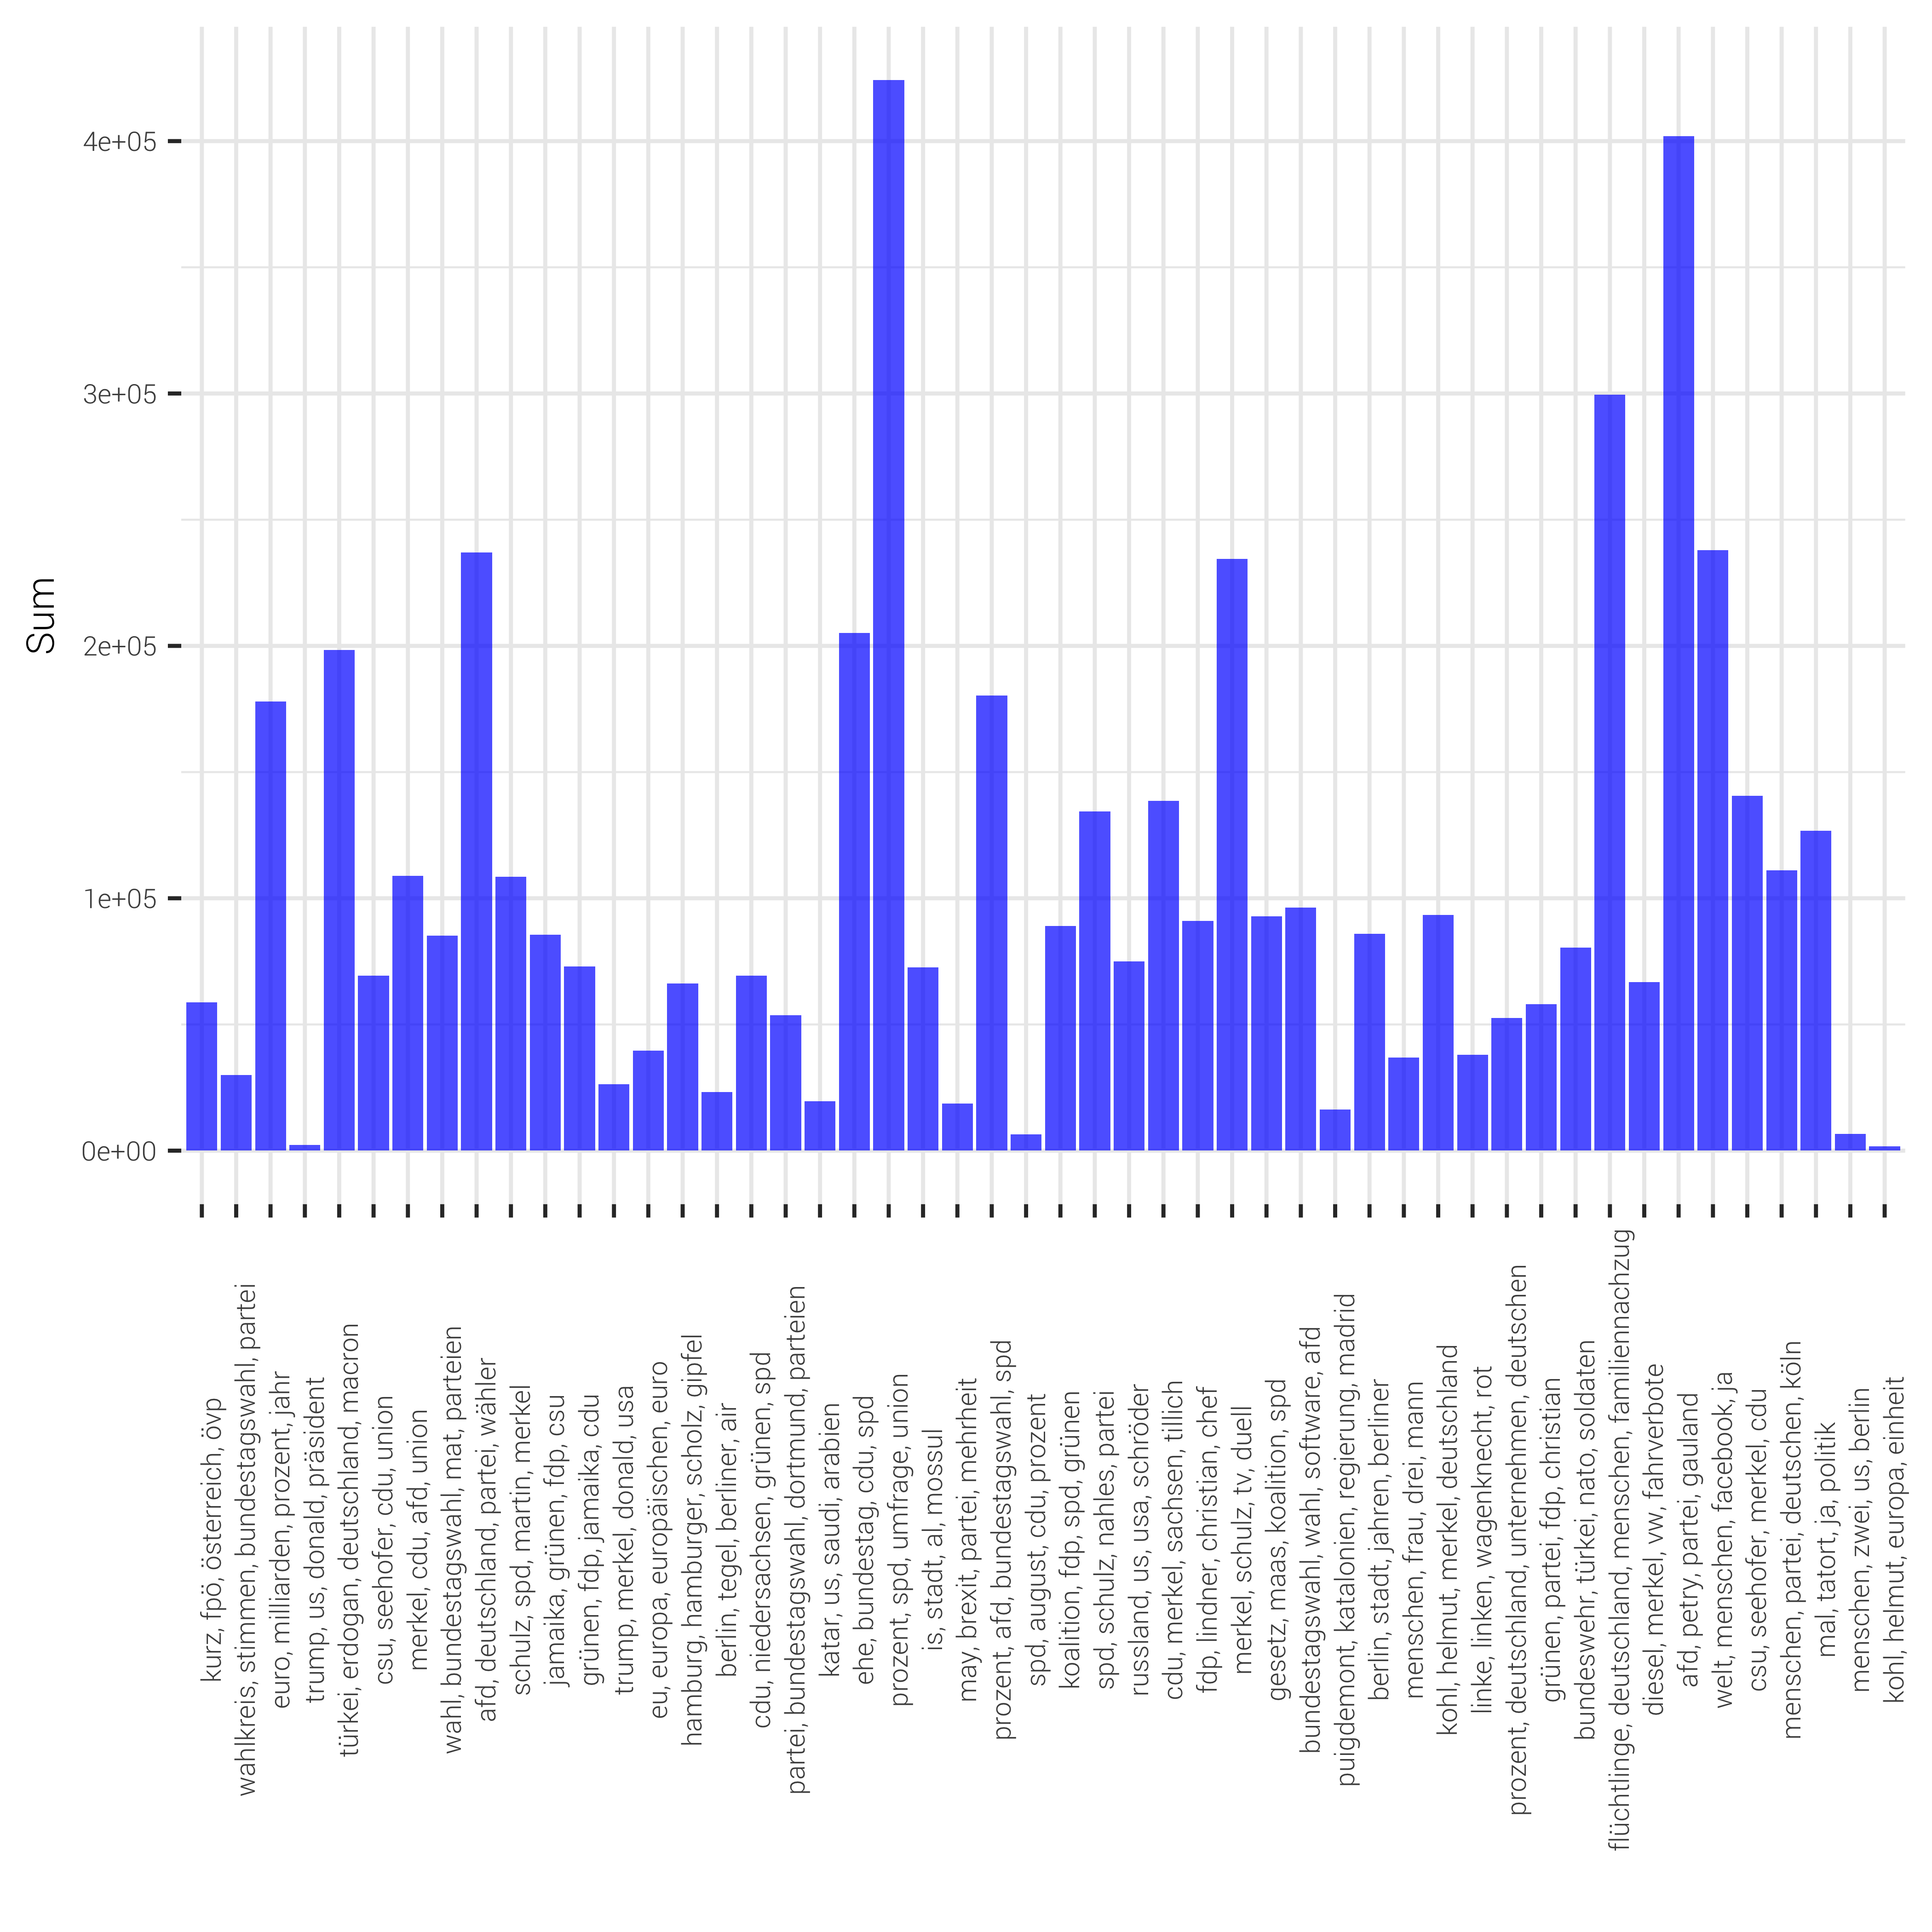
\includegraphics[width=\textwidth]{../figs/fb_shares_topics.png}	
%	\label{fig_fb_shares_topic}
%\end{figure}

In order to answer the primary question of this paper, which topics are more often shared in social networks, we assign a single topic to each article. The examination of the topic probability distribution revealed that most documents are assigned a unique topic with a probability of 50\% and higher (see figure \ref{fig_gamma}), so that we can classify each document based on which topic has the highest probability. We keep only those documents, where the posterior probability of this topic is greater or equal than 0.5 which left us with 6565 documents. Figure \ref{fig_topic_timeline} shows the amount of articles to which a certain topic has been assigned over time. Some of the topics exhibit distinct peaks in the timeline. Topics 11 and 14 deal with the elections, although topic 11 tends to be more about incidents related to the AfD. This graph also illustrates the difference between topic 6 and 17, which have similar labels: topic 6 classifies articles before the negotiations for a "Jamaika" coalition failed, while topic 17 describes the articles written after failure. The highest peak can be found for topic 9, which classifies articles to the riots during the G20 summit. It becomes apparent that more articles deal with riots than with the political content of the summit (topic 8). 

The proportion of zeros in the independent variable (number of Facebook shares) is about 15\%. Figure \ref{fig_fb_shares} reveals that within the bin of 0-1 facebook shares, nearly all articles are published by stern.de. 

\begin{figure}[H]
	\caption{}
	\begin{center}
		\begin{subfigure}[normla]{0.49\textwidth}
			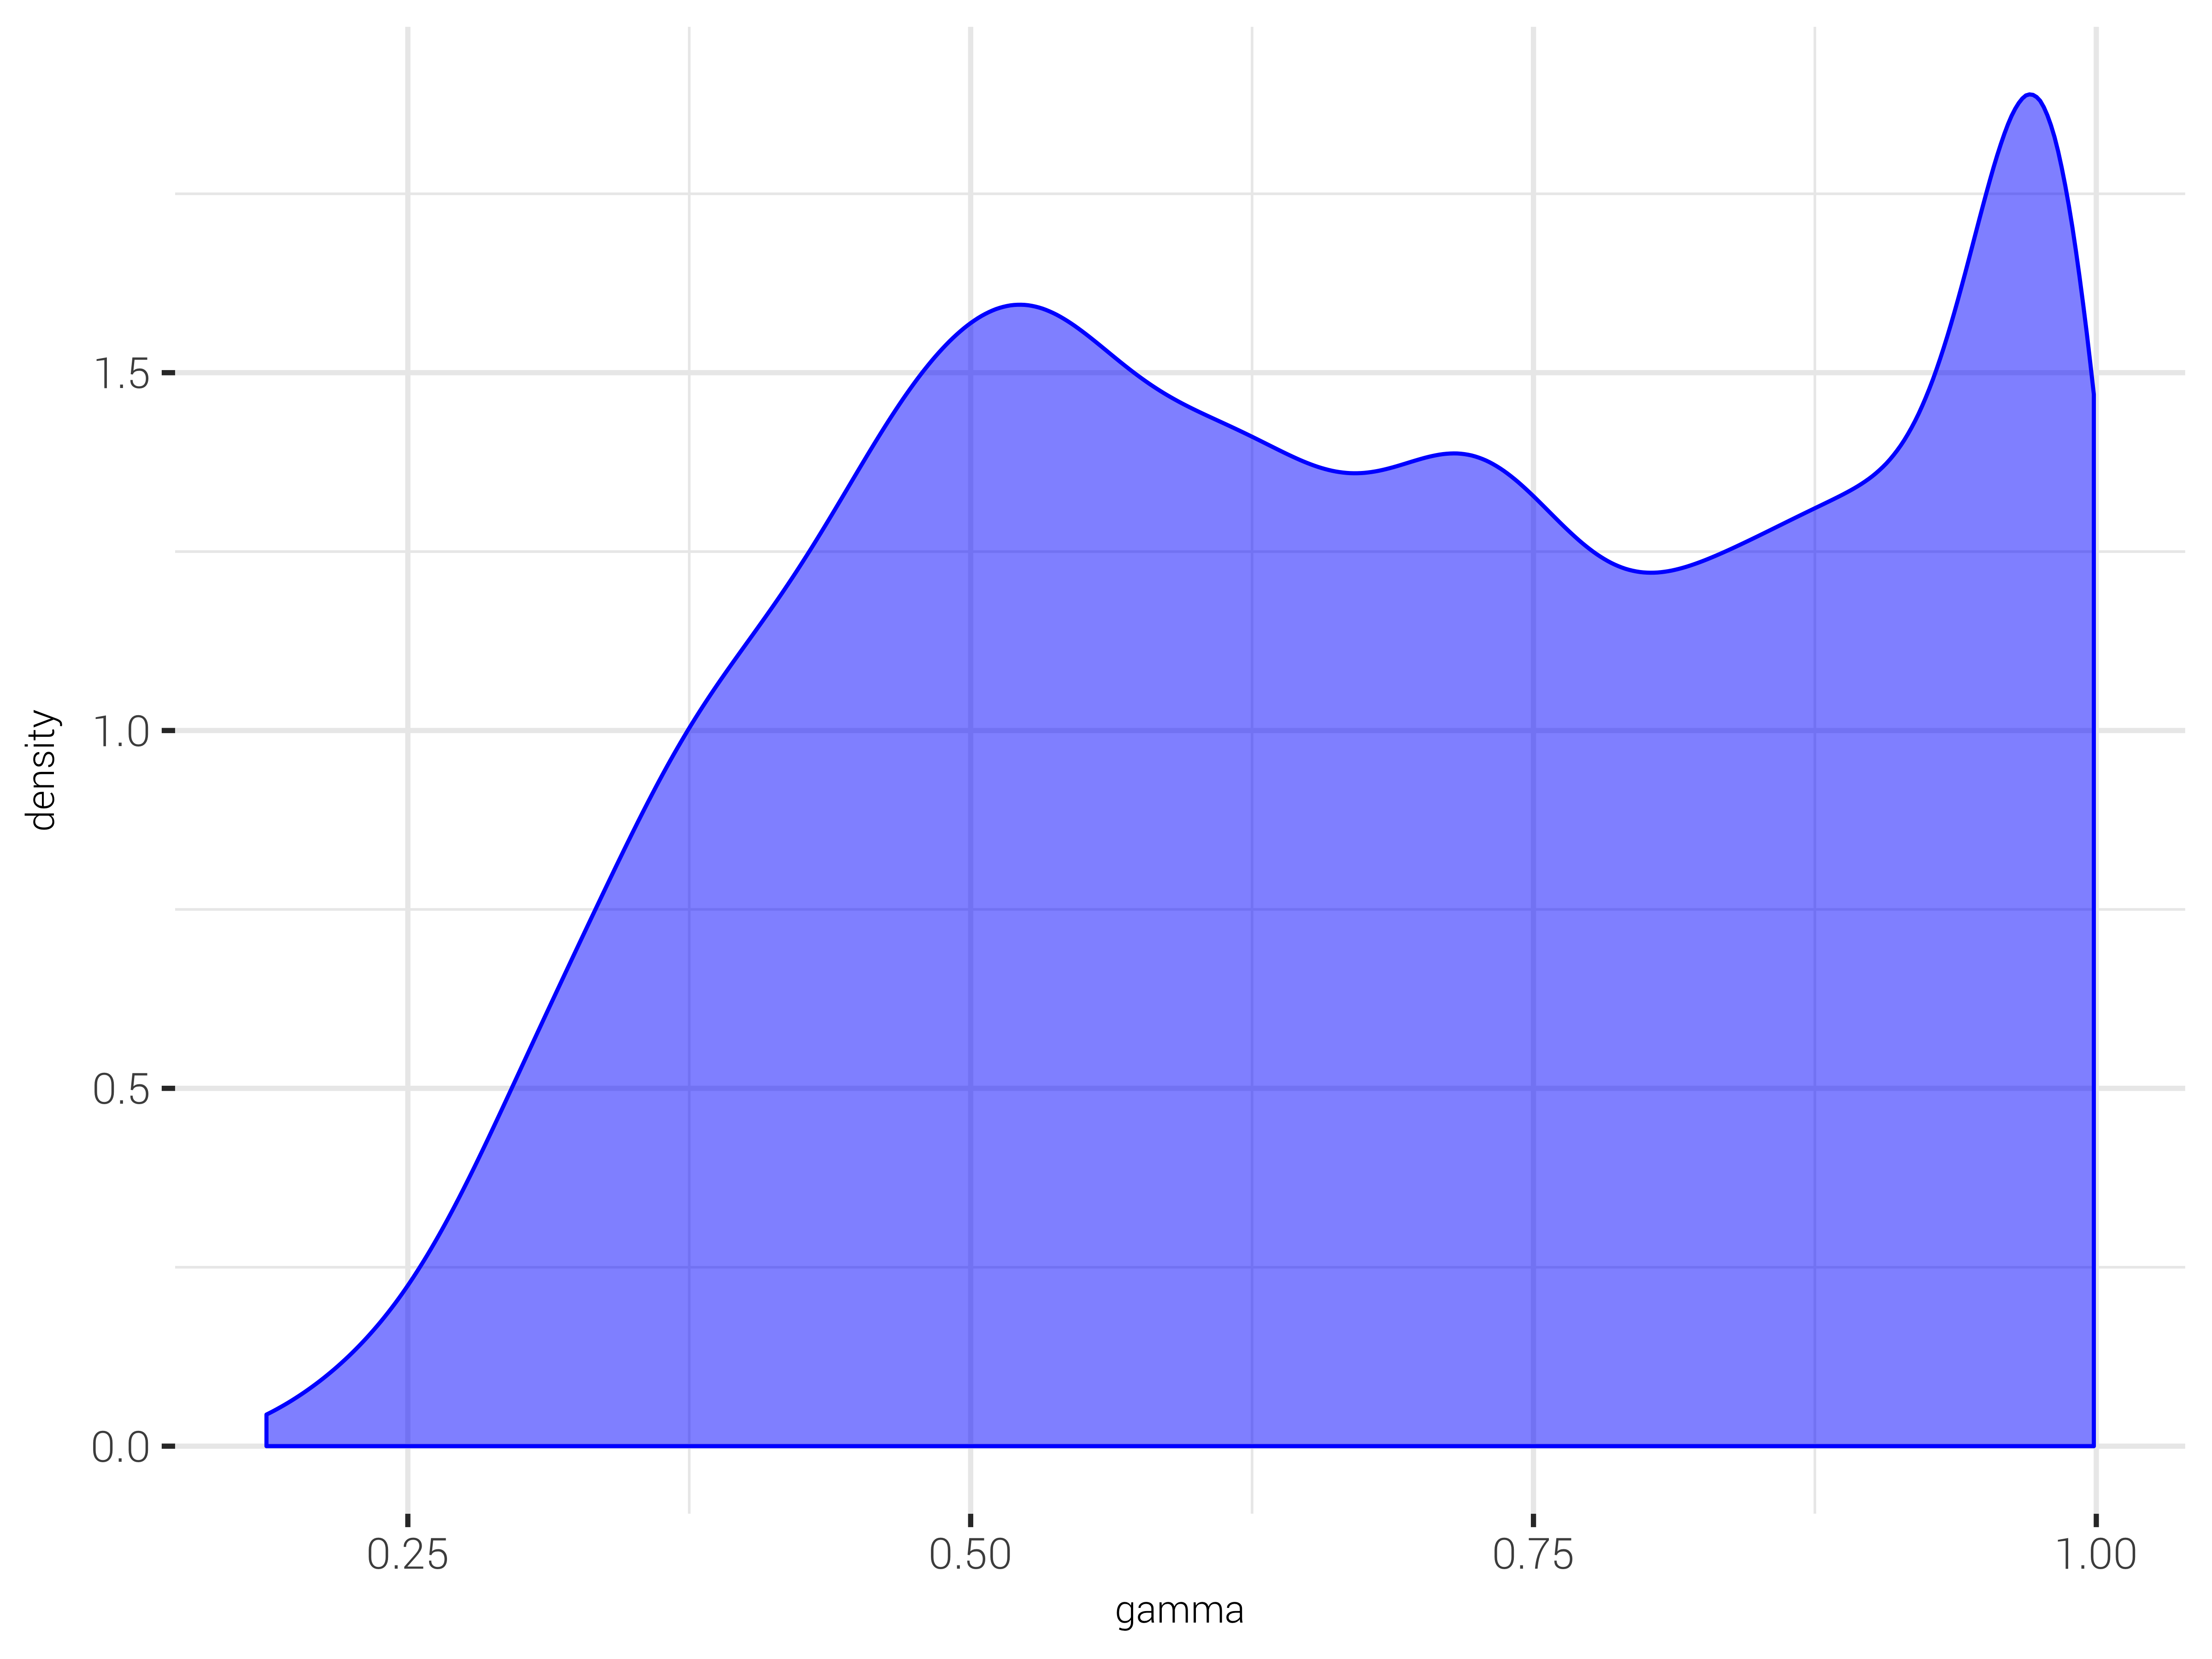
\includegraphics[width=\textwidth,keepaspectratio]{../figs/gamma_dist.png}
			\caption{Density of Top-Topics posterior probability}
			\label{fig_gamma}
		\end{subfigure}
		\begin{subfigure}[normla]{0.49\textwidth}
			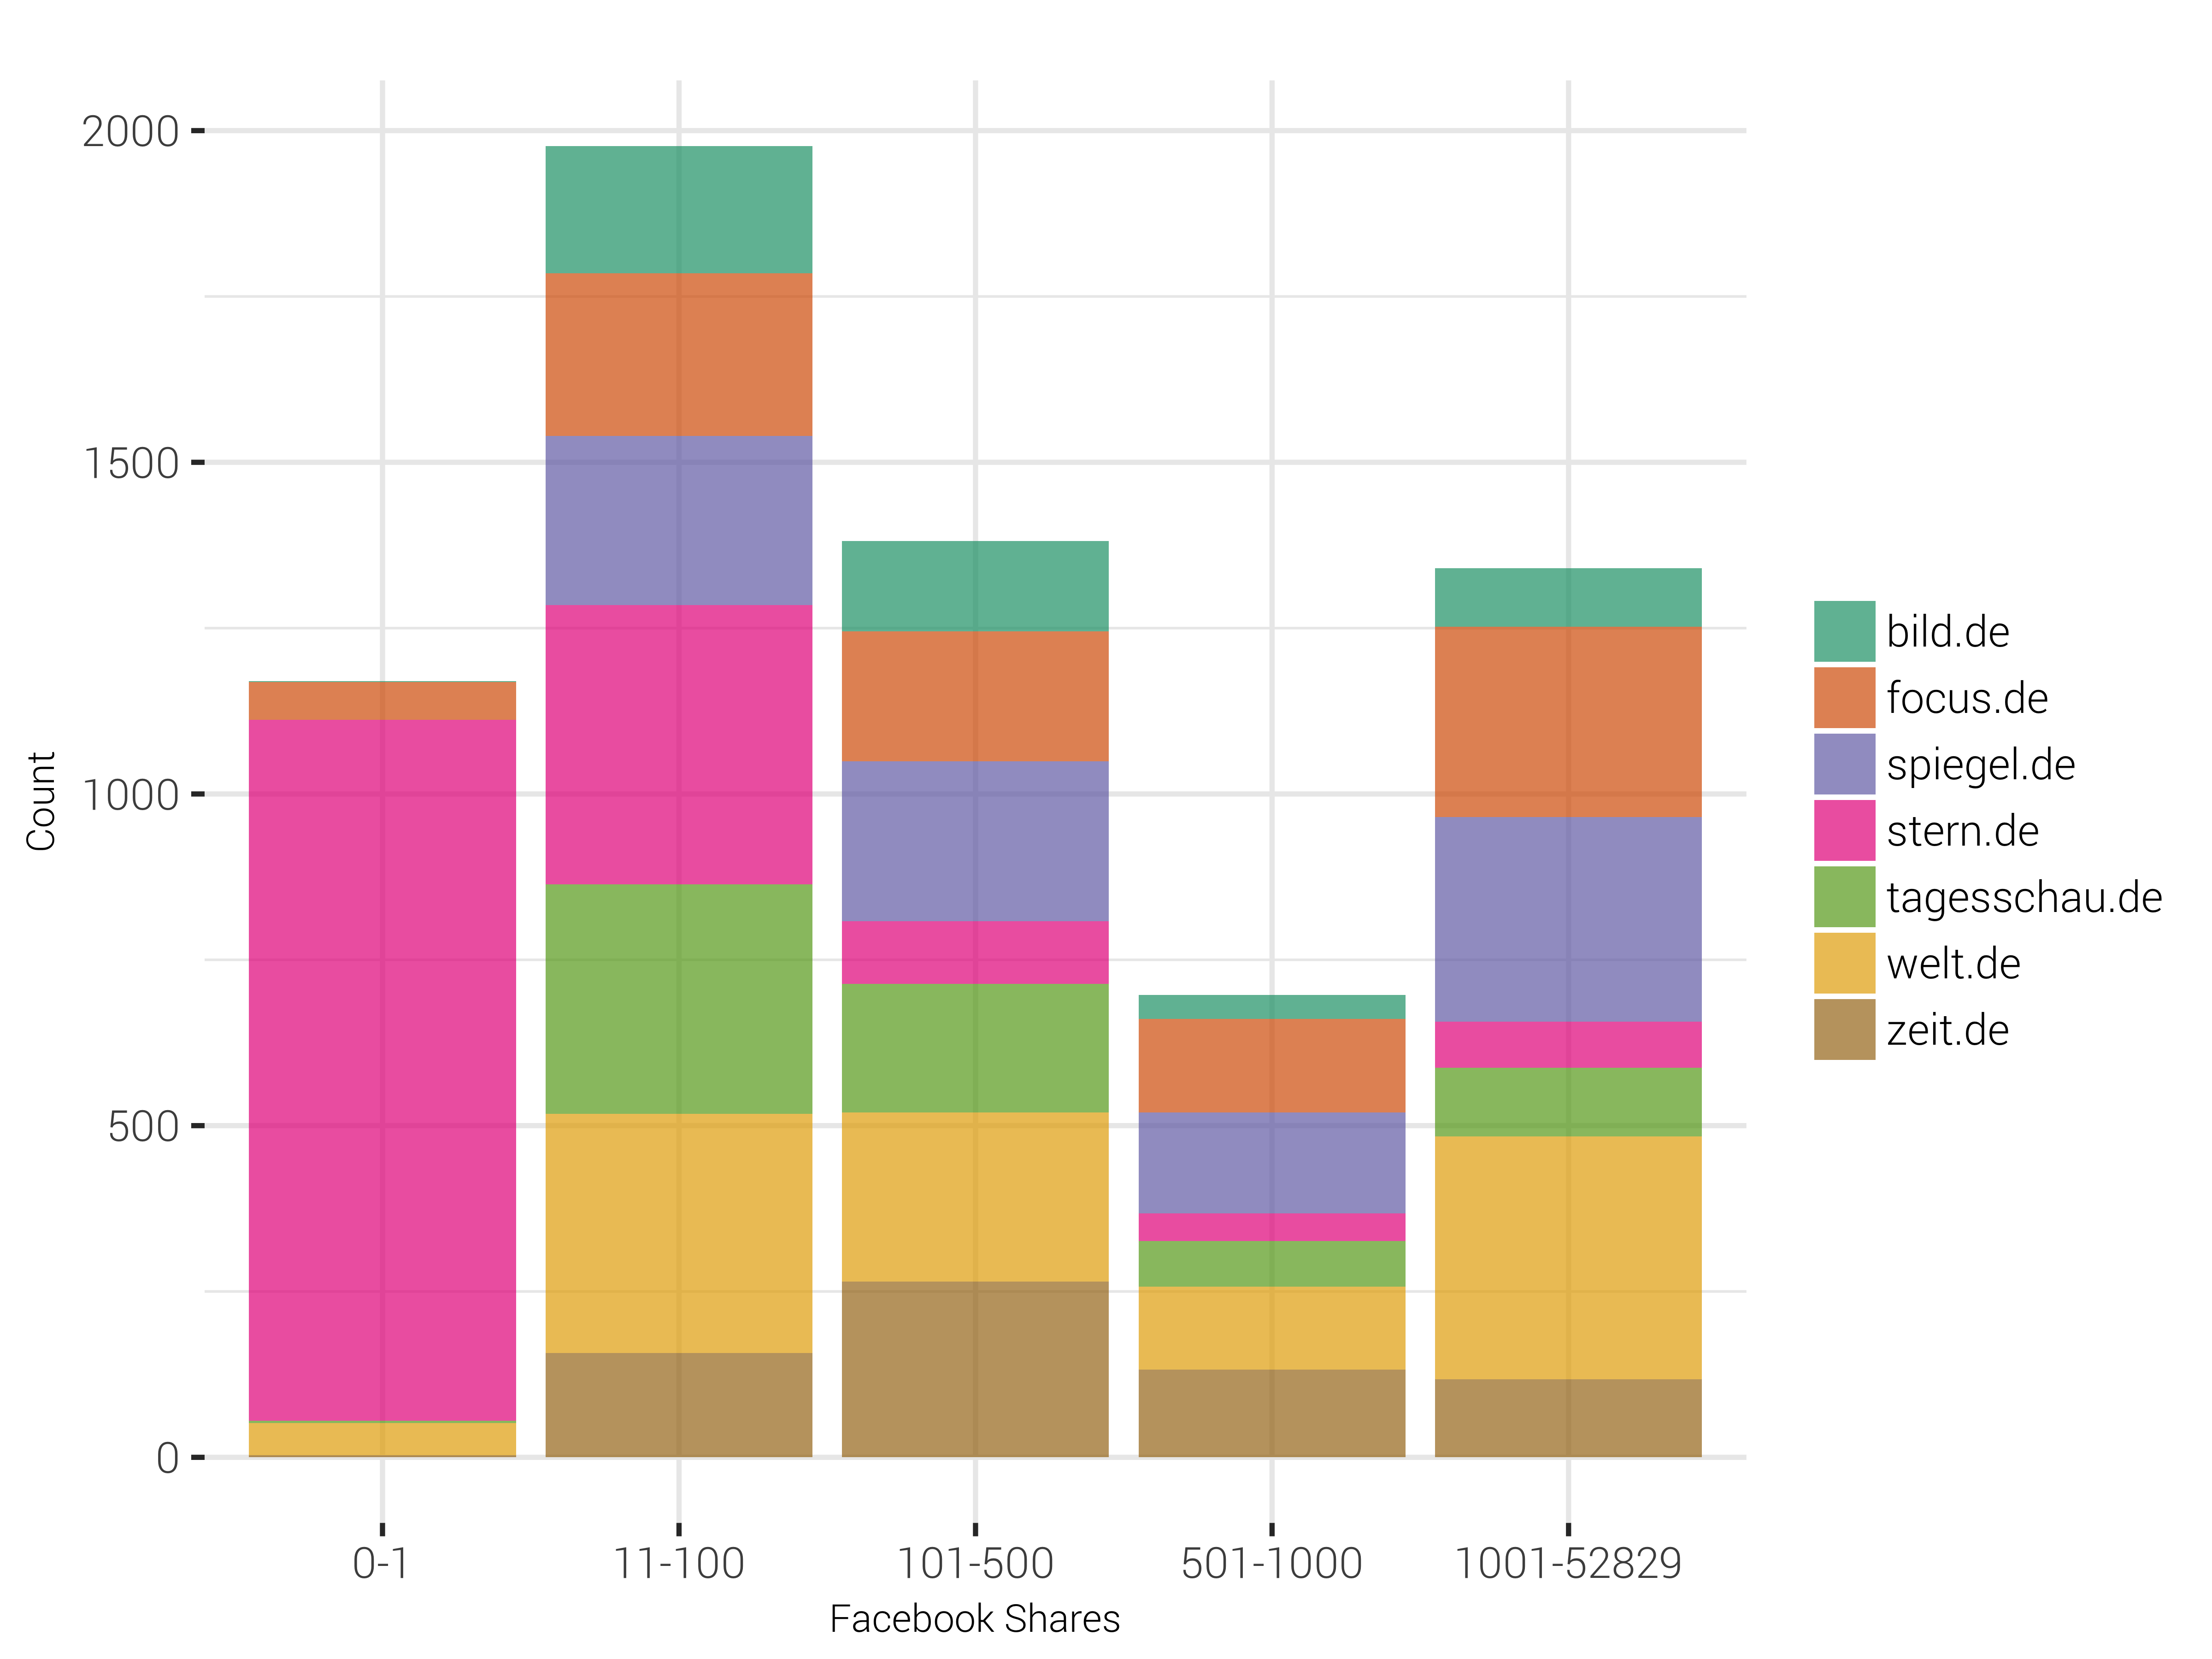
\includegraphics[width=\textwidth,keepaspectratio]{../figs/facebook_shares.png}
			\caption{Grouped Facebook Shares}
			\label{fig_fb_shares}
		\end{subfigure}
		\begin{subfigure}[normla]{0.9\textwidth}
			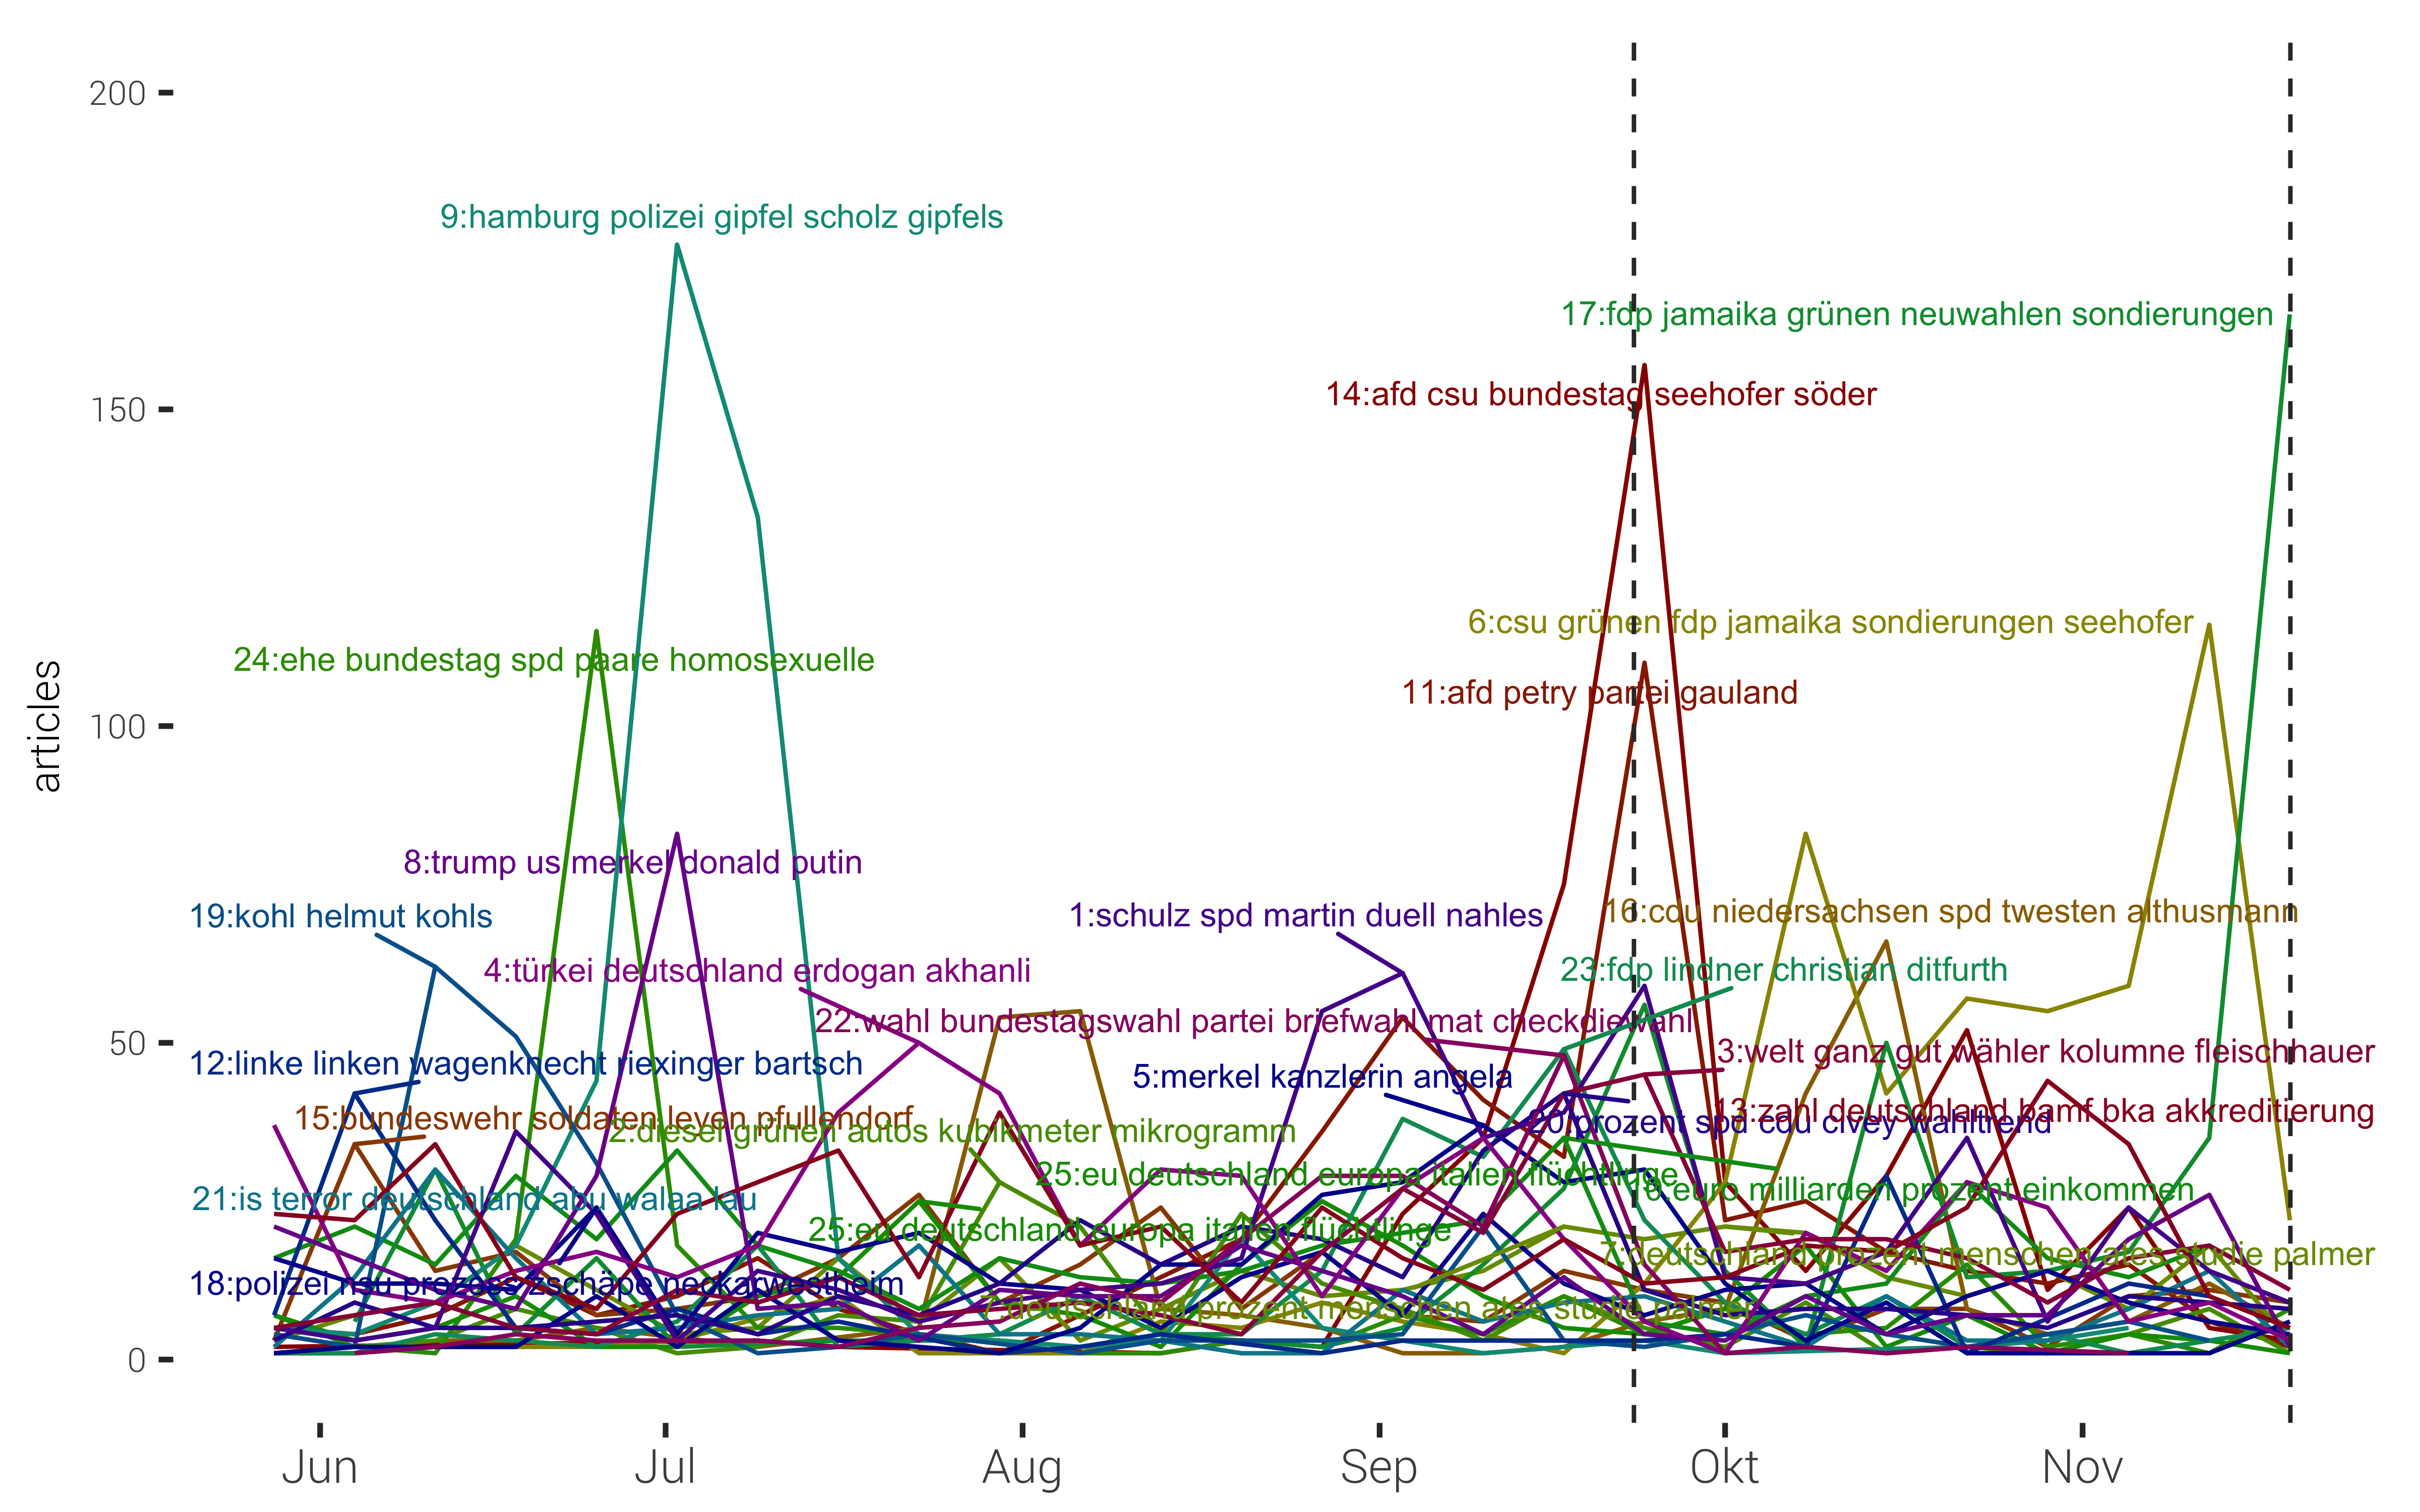
\includegraphics[width=\textwidth,keepaspectratio]{../figs/topic-timeline.png}
			\caption{Topic Timeline}
			\label{fig_topic_timeline}
		\end{subfigure}
	\end{center}
\end{figure}

Model: 

\begin{align*}
	log(FBshares) =\alpha+\beta_{topic}+\beta_{site}+\beta_{textlength}+\epsilon 
\end{align*}


% Table created by stargazer v.5.2 by Marek Hlavac, Harvard University. E-mail: hlavac at fas.harvard.edu
% Date and time: Mi, Dez 06, 2017 - 12:45:38
\begin{table}[!htbp] \centering 
  \caption{} 
  \label{} 
  \begin{adjustbox}{totalheight=\textheight-2\baselineskip}
\begin{tabular}{@{\extracolsep{5pt}}lc} 
\\[-1.8ex]\hline 
\hline \\[-1.8ex] 
 & \multicolumn{1}{c}{\textit{Dependent variable:}} \\ 
\cline{2-2} 
\\[-1.8ex] & fb\_shares\_log \\ 
\hline \\[-1.8ex] 
 topic2 & 0.350$^{*}$ \\ 
  & (0.192) \\ 
  & \\ 
 topic3 & 0.313 \\ 
  & (0.227) \\ 
  & \\ 
 topic4 & 0.533$^{***}$ \\ 
  & (0.159) \\ 
  & \\ 
 topic5 & 0.793$^{***}$ \\ 
  & (0.180) \\ 
  & \\ 
 topic6 & 0.142 \\ 
  & (0.170) \\ 
  & \\ 
 topic7 & $-$0.203 \\ 
  & (0.166) \\ 
  & \\ 
 topic8 & 1.373$^{***}$ \\ 
  & (0.185) \\ 
  & \\ 
 topic9 & 1.040$^{***}$ \\ 
  & (0.153) \\ 
  & \\ 
 topic10 & $-$0.500$^{***}$ \\ 
  & (0.177) \\ 
  & \\ 
 topic11 & $-$0.061 \\ 
  & (0.161) \\ 
  & \\ 
 topic12 & $-$0.565$^{***}$ \\ 
  & (0.187) \\ 
  & \\ 
 topic13 & 0.576$^{***}$ \\ 
  & (0.150) \\ 
  & \\ 
 topic14 & 0.361$^{**}$ \\ 
  & (0.179) \\ 
  & \\ 
 topic15 & $-$0.812$^{***}$ \\ 
  & (0.202) \\ 
  & \\ 
 topic16 & 0.058 \\ 
  & (0.151) \\ 
  & \\ 
 topic17 & 0.311$^{*}$ \\ 
  & (0.186) \\ 
  & \\ 
 topic18 & 0.356$^{*}$ \\ 
  & (0.187) \\ 
  & \\ 
 topic19 & 2.046$^{***}$ \\ 
  & (0.170) \\ 
  & \\ 
 topic20 & 0.0001 \\ 
  & (0.187) \\ 
  & \\ 
 topic21 & 0.934$^{***}$ \\ 
  & (0.161) \\ 
  & \\ 
 topic22 & 0.434$^{**}$ \\ 
  & (0.193) \\ 
  & \\ 
 topic23 & 0.571$^{***}$ \\ 
  & (0.211) \\ 
  & \\ 
 topic24 & 0.975$^{***}$ \\ 
  & (0.170) \\ 
  & \\ 
 topic25 & $-$0.073 \\ 
  & (0.189) \\ 
  & \\ 
 topic26 & 0.258$^{*}$ \\ 
  & (0.152) \\ 
  & \\ 
 topic27 & 0.417 \\ 
  & (0.355) \\ 
  & \\ 
 topic28 & $-$0.067 \\ 
  & (0.194) \\ 
  & \\ 
 siteDIE WELT & 0.389$^{***}$ \\ 
  & (0.112) \\ 
  & \\ 
 siteFOCUS ONLINE & 0.264$^{**}$ \\ 
  & (0.117) \\ 
  & \\ 
 siteSPIEGEL ONLINE & 0.858$^{***}$ \\ 
  & (0.117) \\ 
  & \\ 
 sitestern.de & $-$3.643$^{***}$ \\ 
  & (0.109) \\ 
  & \\ 
 sitetagesschau.de & $-$0.209$^{*}$ \\ 
  & (0.123) \\ 
  & \\ 
 siteZEIT ONLINE & 0.399$^{***}$ \\ 
  & (0.124) \\ 
  & \\ 
 text\_length & 0.0003$^{***}$ \\ 
  & (0.0001) \\ 
  & \\ 
 Constant & 4.594$^{***}$ \\ 
  & (0.148) \\ 
  & \\ 
\hline \\[-1.8ex] 
Observations & 6,743 \\ 
R$^{2}$ & 0.451 \\ 
Adjusted R$^{2}$ & 0.448 \\ 
Residual Std. Error & 2.031 (df = 6708) \\ 
F Statistic & 162.126$^{***}$ (df = 34; 6708) \\ 
\hline 
\hline \\[-1.8ex] 
\textit{Note:}  & \multicolumn{1}{r}{$^{*}$p$<$0.1; $^{**}$p$<$0.05; $^{***}$p$<$0.01} \\ 
\end{tabular}
\end{adjustbox} 
\end{table} 

%
%One way to model this type of situation is to assume that the data come from a mixture of two populations, one where the counts is always zero, and another where the count has a Poisson distribution with mean $\mu$. In this model zero counts can come from either population, while positive counts come only from the second one. 
%
%The distribution of the outcome can then be modeled in terms of two parameters, $\pi$ the probability of 'always zero', and $\mu$, the mean number of publications for those not in the 'always zero' group. A natural way to introduce covariates is to model the logit of the probability $\pi$ of always zero and the log of the mean $\mu$ for those not in the always zero class.
%
%The two-part model relaxes the assumption that the zeros (whether or not the article is shared) and positives (how often it is shared) come from the same data generating process. The zero-inflated model lets the zeros occur in two different ways: as a realization of the binary process (z=0) and as a realization of the count process when the binary variable z=1. 
%
%If the process generating the zeros is $f_1(.)$ and the process generating the positive responses is $f_2(.)$ then the two-part hurdle model is defined by the following probabilities. 
%
%\begin{align*}
%	g(y)=\begin{cases}
%		f_1(0) + 1(f_i(0))f_2(0) if y=0 \\
%		(1-f_1(0))f_2(y) if y\geq 1
%	\end{cases}
%\end{align*}
%
%The model for the zero versus positive responses is a binary model with the specified distribution, but we usually estimate it with the probit/logit model.

% ----------------------
% Appendix
% ----------------------
\section*{Appendix}

\begin{figure}[H]
	\caption{Mean prevalence of topics within each news source corpus 1}
	\begin{center}
		\begin{subfigure}[normla]{0.2\textwidth}
			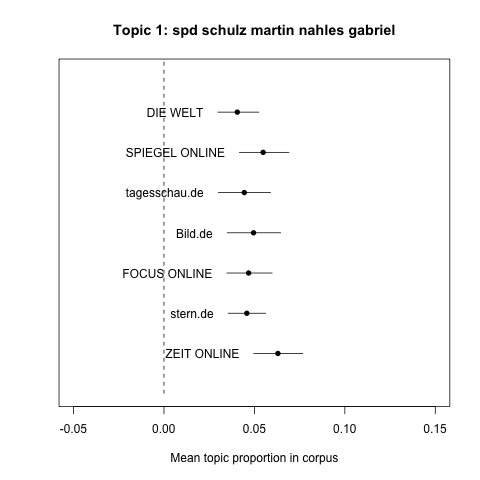
\includegraphics[width=\textwidth]{../figs/estimate_effect1.png}
		\end{subfigure}
		\begin{subfigure}[normla]{0.2\textwidth}
			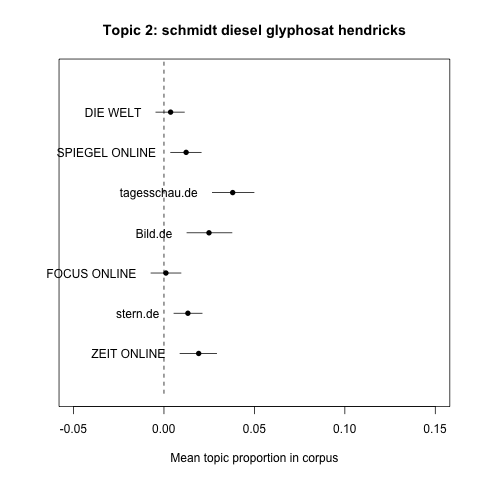
\includegraphics[width=\textwidth]{../figs/estimate_effect2.png}
		\end{subfigure}
				\begin{subfigure}[normla]{0.2\textwidth}
			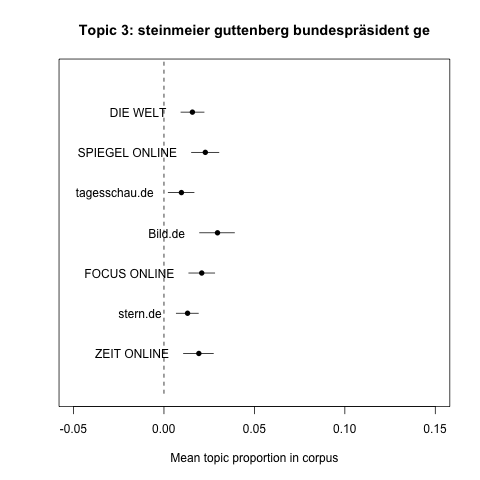
\includegraphics[width=\textwidth]{../figs/estimate_effect3.png}
		\end{subfigure}
				\begin{subfigure}[normla]{0.2\textwidth}
			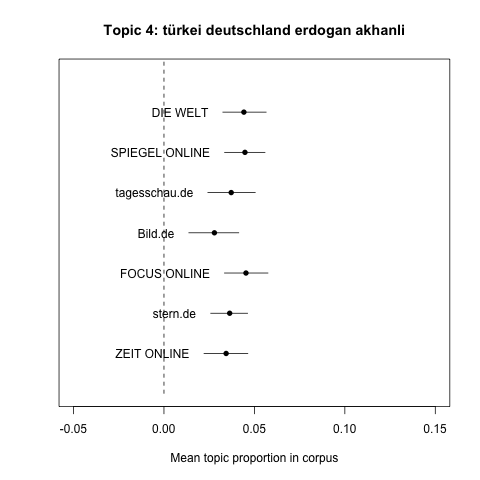
\includegraphics[width=\textwidth]{../figs/estimate_effect4.png}
		\end{subfigure}
				\begin{subfigure}[normla]{0.2\textwidth}
			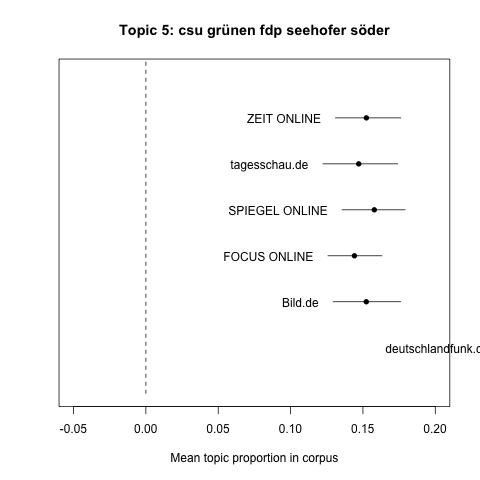
\includegraphics[width=\textwidth]{../figs/estimate_effect5.png}
		\end{subfigure}
				\begin{subfigure}[normla]{0.2\textwidth}
			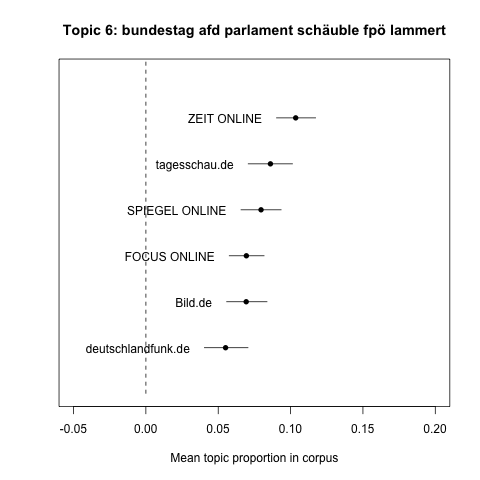
\includegraphics[width=\textwidth]{../figs/estimate_effect6.png}
		\end{subfigure}
		\begin{subfigure}[normla]{0.2\textwidth}
			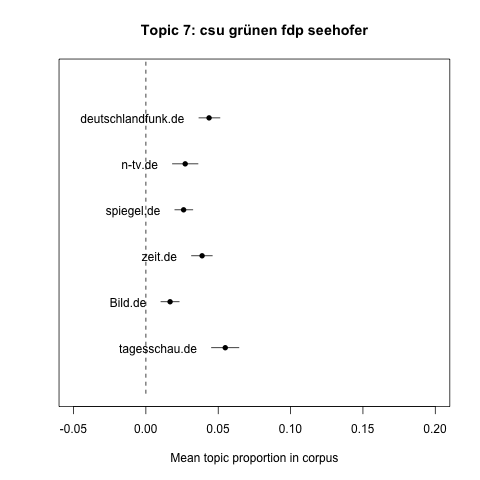
\includegraphics[width=\textwidth]{../figs/estimate_effect7.png}
		\end{subfigure}
		\begin{subfigure}[normla]{0.2\textwidth}
			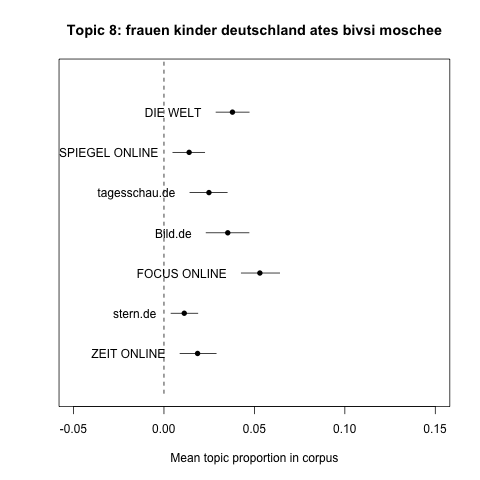
\includegraphics[width=\textwidth]{../figs/estimate_effect8.png}
		\end{subfigure}
		\begin{subfigure}[normla]{0.2\textwidth}
			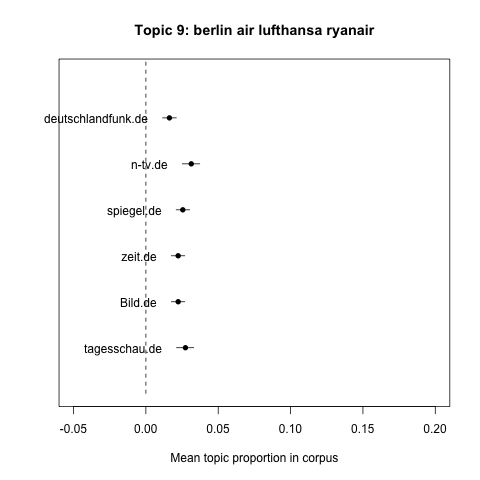
\includegraphics[width=\textwidth]{../figs/estimate_effect9.png}
		\end{subfigure}
		\begin{subfigure}[normla]{0.2\textwidth}
			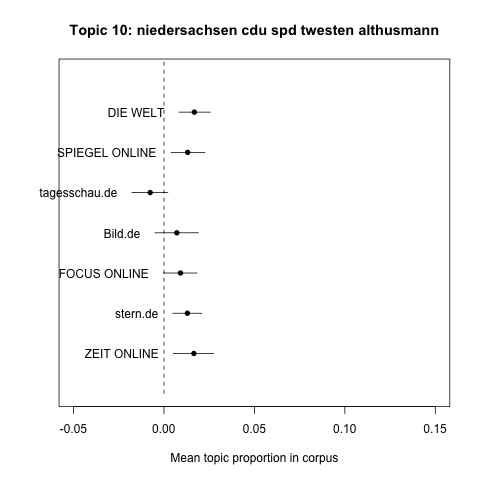
\includegraphics[width=\textwidth]{../figs/estimate_effect10.png}
		\end{subfigure}
		\begin{subfigure}[normla]{0.2\textwidth}
			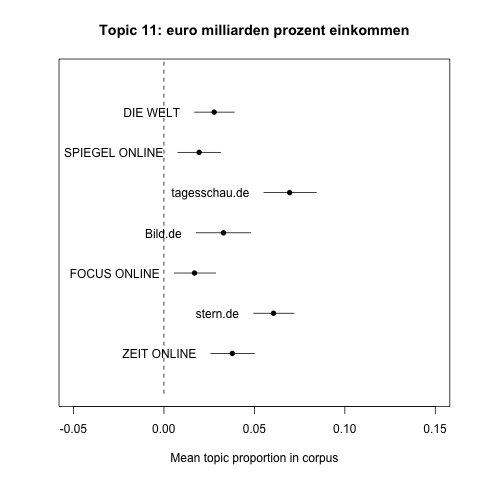
\includegraphics[width=\textwidth]{../figs/estimate_effect11.png}
		\end{subfigure}
		\begin{subfigure}[normla]{0.2\textwidth}
			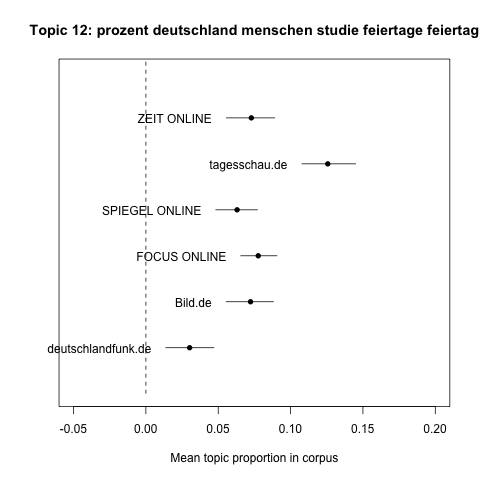
\includegraphics[width=\textwidth]{../figs/estimate_effect12.png}
		\end{subfigure}
		\begin{subfigure}[normla]{0.2\textwidth}
			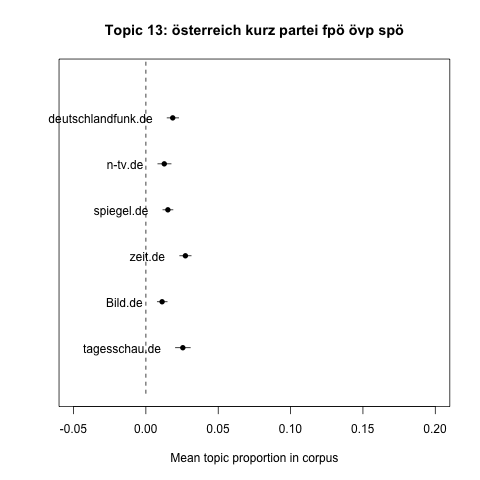
\includegraphics[width=\textwidth]{../figs/estimate_effect13.png}
		\end{subfigure}
		\begin{subfigure}[normla]{0.2\textwidth}
			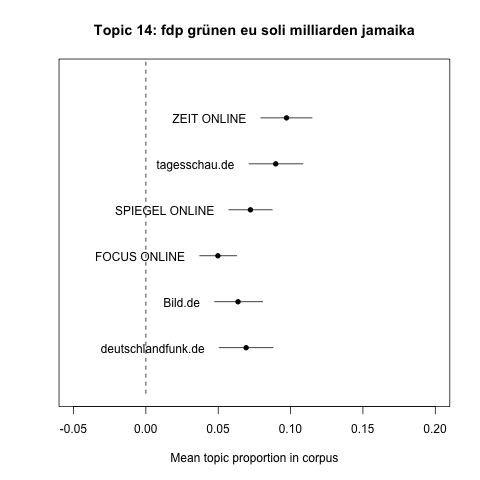
\includegraphics[width=\textwidth]{../figs/estimate_effect14.png}
		\end{subfigure}
	\end{center}
	\label{fig_estimateEffects_full1}
\end{figure}

\begin{figure}[H]
	\caption{Mean prevalence of topics within each news source corpus 2}
	\begin{center}
			\begin{subfigure}[normla]{0.2\textwidth}
			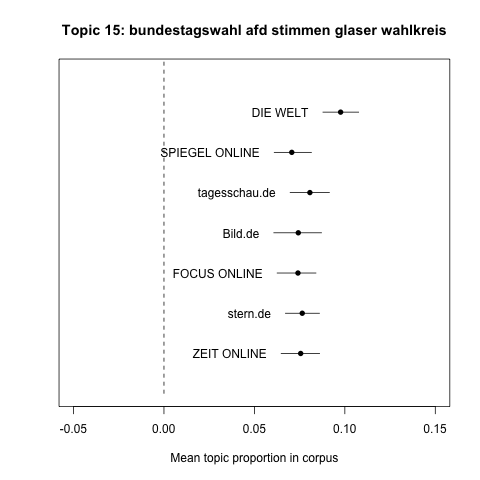
\includegraphics[width=\textwidth]{../figs/estimate_effect15.png}
		\end{subfigure}
		\begin{subfigure}[normla]{0.2\textwidth}
			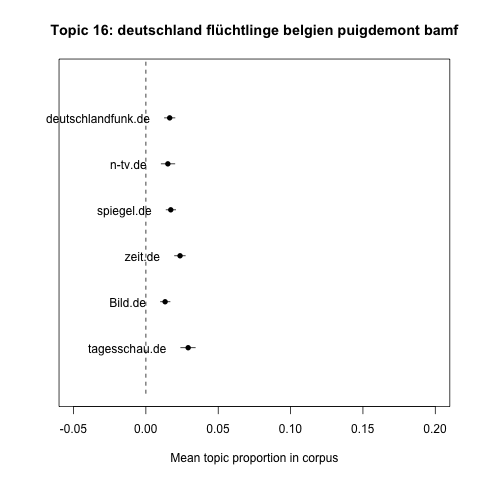
\includegraphics[width=\textwidth]{../figs/estimate_effect16.png}
		\end{subfigure}
		\begin{subfigure}[normla]{0.2\textwidth}
			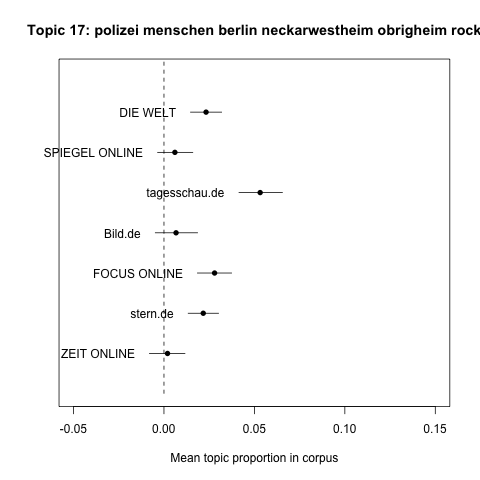
\includegraphics[width=\textwidth]{../figs/estimate_effect17.png}
		\end{subfigure}
		\begin{subfigure}[normla]{0.2\textwidth}
			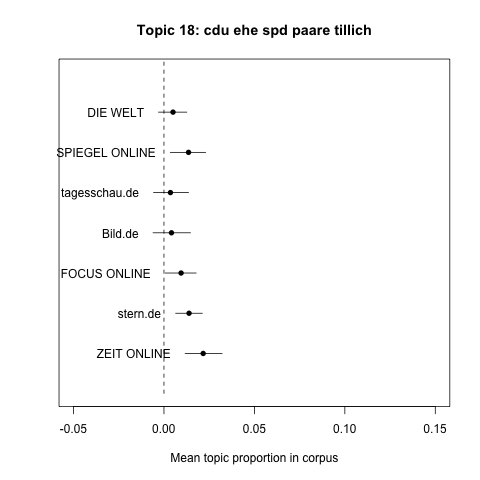
\includegraphics[width=\textwidth]{../figs/estimate_effect18.png}
		\end{subfigure}
		\begin{subfigure}[normla]{0.2\textwidth}
			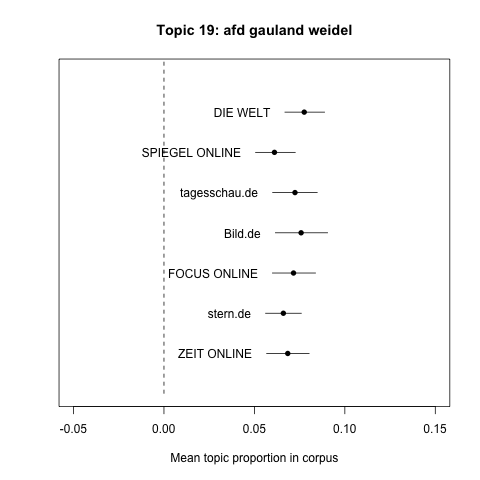
\includegraphics[width=\textwidth]{../figs/estimate_effect19.png}
		\end{subfigure}
		\begin{subfigure}[normla]{0.2\textwidth}
			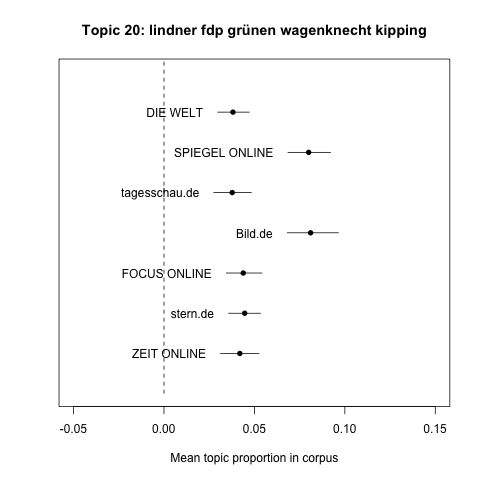
\includegraphics[width=\textwidth]{../figs/estimate_effect20.png}
		\end{subfigure}
		\begin{subfigure}[normla]{0.2\textwidth}
			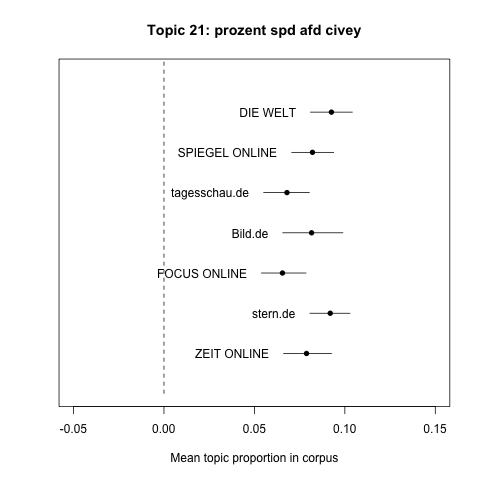
\includegraphics[width=\textwidth]{../figs/estimate_effect21.png}
		\end{subfigure}
		\begin{subfigure}[normla]{0.2\textwidth}
			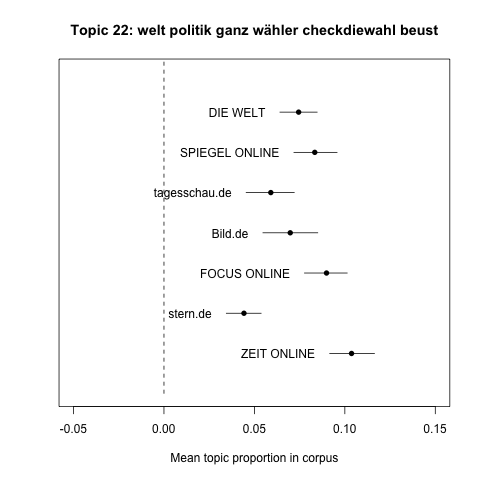
\includegraphics[width=\textwidth]{../figs/estimate_effect22.png}
		\end{subfigure}
		\begin{subfigure}[normla]{0.2\textwidth}
			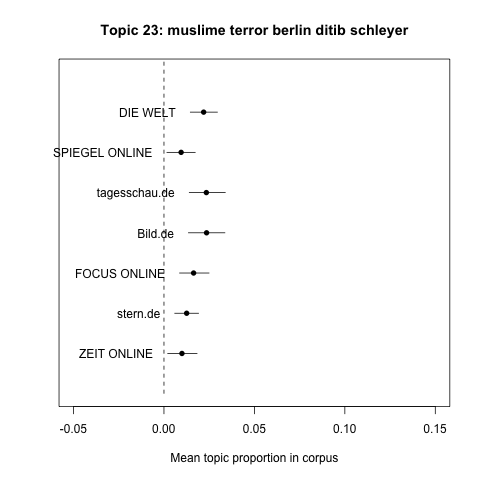
\includegraphics[width=\textwidth]{../figs/estimate_effect23.png}
		\end{subfigure}
		\begin{subfigure}[normla]{0.2\textwidth}
			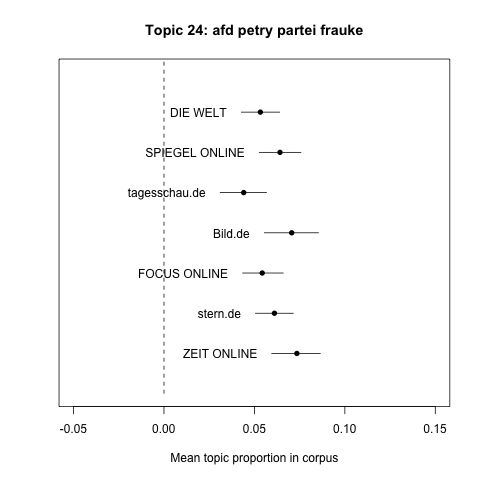
\includegraphics[width=\textwidth]{../figs/estimate_effect24.png}
		\end{subfigure}
		\begin{subfigure}[normla]{0.2\textwidth}
			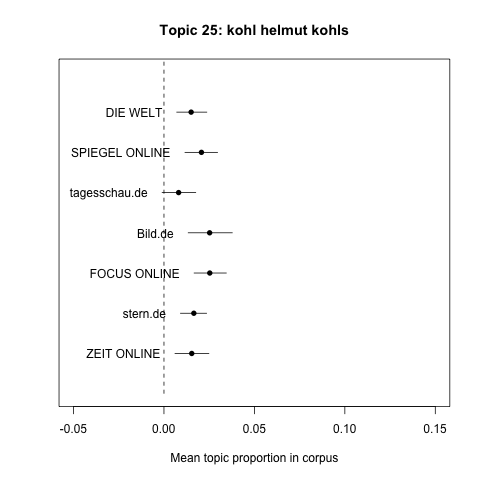
\includegraphics[width=\textwidth]{../figs/estimate_effect25.png}
		\end{subfigure}
		\begin{subfigure}[normla]{0.2\textwidth}
			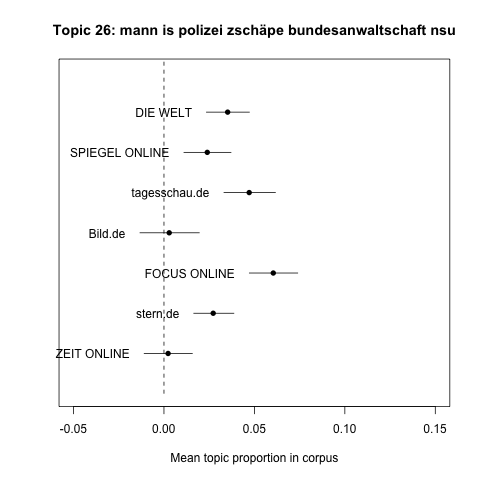
\includegraphics[width=\textwidth]{../figs/estimate_effect26.png}
		\end{subfigure}
				\begin{subfigure}[normla]{0.2\textwidth}
			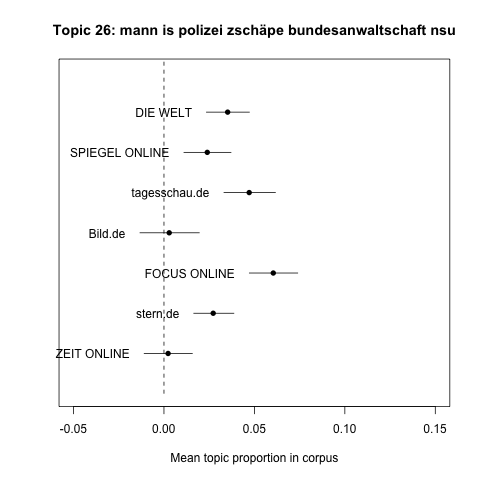
\includegraphics[width=\textwidth]{../figs/estimate_effect26.png}
		\end{subfigure}
				\begin{subfigure}[normla]{0.2\textwidth}
			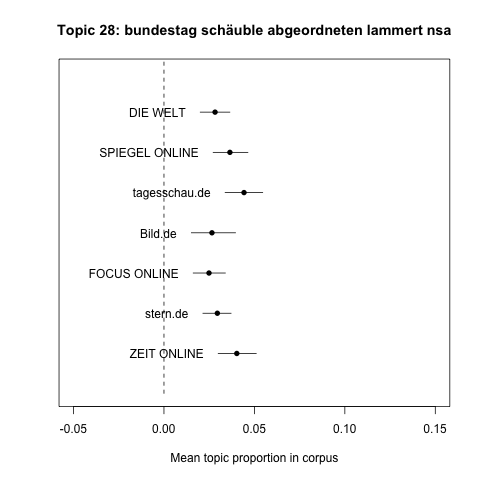
\includegraphics[width=\textwidth]{../figs/estimate_effect28.png}
		\end{subfigure}
	\end{center}
	\label{fig_estimateEffects_full2}
\end{figure}

\end{document}
